\documentclass[12pt, a4paper, oneside]{book}


%------------------------
% IMPORT PACKAGES
%-----------------------
\usepackage{amsthm}
\usepackage{mathtools}
\usepackage{algpseudocode}
\usepackage[chapter]{algorithm}
\usepackage{amssymb}
\usepackage{graphicx}
\usepackage{caption}
\usepackage{fancyvrb}
\usepackage{array}
\usepackage[gen]{eurosym}
\usepackage{cancel}
\usepackage{multicol}
\usepackage[acronym,toc,nohypertypes={acronym,notation},nonumberlist,automake]{glossaries}
%\usepackage{hyperref}
\usepackage{epigraph}
\usepackage{url}
\def\UrlBreaks{\do\/\do-}
\usepackage{breakurl}
\usepackage[breaklinks]{hyperref}

%% remark theoremstyle
%\newtheoremstyle{break}
%{\topsep}{\topsep}%
%{\itshape}{}%
%{\bfseries}{}%
%{\newline}{}%
%\theoremstyle{break}
%\newtheorem{remark}{Remark}[section]

% problem theoremstyle
%\newtheoremstyle{problemstyle}  % <name>
%{10pt}  % <space above>
%{10pt}  % <space below>
%{\normalfont} % <body font>
%{}  % <indent amount}
%{\bfseries\itshape} % <theorem head font>
%{\normalfont\bfseries:} % <punctuation after theorem head>
%{.5em} % <space after theorem head>
%{} % <theorem head spec (can be left empty, meaning `normal')>
%\theoremstyle{problemstyle}
%\newtheorem{problem}{Problem}[section] % Comment out [section] toremove section number dependence
%\newtheorem{definition}{Definition}[section]
%\newtheorem{theorem}{Theorem}[section]
%\newtheorem{proposition}{Proposition}[section]
%\newtheorem{remark}{Remark}[section]
%\newtheorem{lemma}{Lemma}[section]
% create command for variance in math mode
%\newcommand{\Var}[1]{\operatorname{Var}\left[#1\right]}
\newtheorem{mydef}{Definition}[section]
\newtheorem{myrem}{Remark}[section]
\newtheorem{myexample}{Example}[section]
\newtheorem{myprop}{Proposition}[section]
\newtheorem{mylemma}{Lemma}[section]
\newtheorem{mytheorem}{Theorem}[section]

\renewcommand{\labelitemii}{$\bullet$}
\renewcommand\textflush{flushright}
\setlength\epigraphwidth{.6\textwidth}
\newcommand{\source}[1]{\caption*{Source: {#1}} }

\makeglossaries
\newacronym{}{}{}





\begin{document}


%----------------------------------------------------------------------------------------
% COVER PAGE
%----------------------------------------------------------------------------------------
\pagestyle{empty}
\begin{titlepage}

	\begin{center}
		\normalsize 
			\textsc{Politecnico di Milano}\\
			Scuola di Ingegneria Industriale e dell'Informazione\\
      		Corso di Laurea Magistrale in Ingegneria Matematica\\
	\end{center}
	\vspace{.6cm}
	
	\begin{figure}[htpb]
		\centering
		
\includegraphics[width=4cm]{Cover/polimi}
	\end{figure}
	\vspace{.6cm}
	
	\begin{center}
		\LARGE
			\textsc{Addressing Privacy and Fungibility Issues in Bitcoin: Confidential Transactions}
	\end{center}
	\vspace{1.6cm}

	\begin{flushleft}
		\large
		\begin{tabular}{ll}
		Relatori:    & Prof. Daniele MARAZZINA      \\
		             & Prof. Ferdinando Maria AMETRANO
		\end{tabular}
		\vspace{1cm}
	\end{flushleft}
	
	\begin{flushright}
		\large
		Tesi di Laurea di:\\
		Alessandro MIOLA\\
		Matr. 862753\\		
	\end{flushright}
	
	\vspace*{\fill}
	\begin{center}
		Anno Accademico 2017-2018
	\end{center}
	
\end{titlepage}


%----------------------------------------------------------------------------------------
% ABSTRACT
%---------------------------------------------------------------------------------------

%% Set page numbers of the introduction to roman  
\frontmatter
\pagestyle{plain}
%\chapter{Abstract}
\label{chpr:abstract}
Insufficient privacy is recognized to be one of the major vulnerabilities of the Bitcoin's protocol, even because it undermines its fungibility. Bitcoin eliminates the need for a trusted third party, but mainly faces users' privacy by hiding them behind pseudonymous addresses.\\
This work aims at presenting \textit{confidential transactions}, the first proposal for a transaction format with encrypted amounts in Bitcoin, which would strongly increase value privacy. It exploits homomorphic encryption which does not remarkably hurt universal validation of transactions, a crucial premise for the achievement of a distributed consensus on the order of valid transactions.

%\cleardoublepage
\vspace*{\fill}
\epigraph{\textit}{}{}
\vspace*{\fill}


%----------------------------------------------------------------------------------------
%	LIST OF CONTENTS/FIGURES/TABLES PAGES
%----------------------------------------------------------------------------------------

\tableofcontents
\listoftables
\addcontentsline{toc}{chapter}{List of Tables}
\listoffigures
\addcontentsline{toc}{chapter}{List of Figures}
\listofalgorithms
\addcontentsline{toc}{chapter}{List of Algorithms}
\printglossaries

\chapter{Abstract}
\label{chpr:abstract}
Insufficient privacy is recognized to be one of the major vulnerabilities of the Bitcoin's protocol, even because it undermines its fungibility. Bitcoin eliminates the need for a trusted third party, but mainly faces users' privacy by hiding them behind pseudonymous addresses.\\
This work aims at presenting \textit{confidential transactions}, the first proposal for a transaction format with encrypted amounts in Bitcoin, which would strongly increase value privacy. It exploits homomorphic encryption which does not remarkably hurt universal validation of transactions, a crucial premise for the achievement of a distributed consensus on the order of valid transactions.
\chapter{Acknowledgements}
\label{chpr:acknowledgement}
First of all, I would like to thank my thesis supervisors: Prof. Ferdinando Ametrano for having shared his passion for the subject and knowledge with me and Prof. Daniele Marazzina for his precious advices during the drawing up phase.\\ \ \\
Then, I would like to express my profound gratitude to my parents and Albi for having always been by my side: mum, for for having taught to me that gentle manners always win, for her sensibility and for being mum (it is difficult to say it otherwise!); dad, for having wisely taught to me that anything can be reached with commitment and determination and for all the efforts spent in helping me become a better man; Albi for having turned bad days with a smile or a joke. And a big thank goes to my grandparents too, for having always supported me despite the distance.\\ \ \\
Furthermore, I would like to thank my high school friends. Having encountered all of you has been a great gift. In particular, Gio (the nicest man I know), the great Lollo and the wise Luca. And again Ambra, Anna, Chiara, Cicchi, Genna, Marti, Massi, Miks and Ventu.\\ \ \\
Finally, a special thanks also goes to the great friends met at university. First of all to Dodo, Gallo, Gigi, Giulio, Gugo, Michi, Simo and Teo. These years would have been even harder without you. And again to Antea, Pietro, Richi and many others I had the opportunity to meet and work with.\\ \ \\
Thank you all.



%----------------------------------------------------------------------------------------
%	THESIS CONTENT - CHAPTERS
%----------------------------------------------------------------------------------------

\mainmatter

\chapter{Introduction}
\label{chpr:intro}

\section{Structure}

\chapter{Privacy and fungibility issues in Bitcoin}
\label{chpr:priv_fung}
Traditional, centralized financial institutions provide a level of privacy in their systems with respect to the outside world which is necessary for personal and commercial reasons at first (to preserve the freedom to transact, not to let commercial competitors monitor your own activity). The obvious concern, however, is that this level of privacy is not guaranteed against the same institutions providing the service and this opens a lot of issues regarding data collection and data privacy. \\
Bitcoin's breakthrough to have succeeded in building a decentralized distributed network where distributed consensus is reached among the nodes of the network has put some constraints on the underlying security model which seem to conflict with the privacy issues addressed above. However this is quite unavoidable: whereas decentralized systems are easy to build without consensus and, on the other hand, consensus is easy to achieve in centralized systems, maintaining both properties in the same system proves to be a hard challenge.\\ 
Bitcoin's security model is based on the achievement of distributed consensus which in turn requires (among the others) universal and independent verification of the validity of each transaction, made possible by having public transaction data. That is, transparency is needed to obtain and strengthen security.\\
This lack of privacy is recognized to be a weak point within the Bitcoin's protocol and several proposals to improve different aspects of privacy in Bitcoin have appeared in the years, despite never being effectively softforked. The main reason for this being basically the high costs that the massive adoption for privacy-based solutions would imply: privacy is costly and requires commitments. Nevertheless, advances in monitoring capabilities of the blockchain, newborn businesses in Bitcoin blockchain's analysis urge the need for privacy-based solutions in the long run.\\
The original protocol has addressed the problem mainly through the adoption of pseudonymous addresses, that on one hand seem robust if one does not know who owns which addresses, but suffer both from some unsafe users practices (like address reuse) and from the possibility to exploit coins linkability\footnote{The need of a user to generally spend the change back to himself when transacting (due to transaction outputs generally not embedding the right value to be spent in a successive transaction) basically links transaction outputs and so addresses. Moreover in case previously collected changes are too small to cover a transaction output in its entirety, this makes it necessary to combine changes and so further linking transactions.} to trace the transaction graph.\\
Instead, a point in favour of having less privacy and more transparency comes from whom is mainly concerned with the use of cryptocurrencies like bitcoin for illicit activities, who argues that this could be a feature that can help investigations.
\section{Types of privacy in Bitcoin}
\label{sec::priv_1}
Due to how the Bitcoin's protocol has been conceived and implemented, the aim to strengthen privacy should regard different aspects whose improvement can be beneficial. In particular, the concern should be at least on \textit{association} privacy, \textit{balance} privacy, \textit{identity} privacy and \textit{transaction value} privacy.\\
Improving association privacy would mean enhancing transaction graph privacy not letting the possibility to understand who is paying who, thus addressing the previously discussed linkage between transactions and making transaction graph analysis harder. A typical practice undermining it is address reuse, that is however nowadays reduced by wallets using a Hierarchical Deterministic derivation of keys (and so addresses). Moreover, different solutions have been proposed in this field in the years. We present the idea behind only some of them, but it is worth to notice that solutions trying to address association privacy are many more.\\ One of the first is Coinjoin \cite{Max13}, which starts from the important premise that when a transaction spends from multiple addresses it is not necessarily the case that these addresses all come from the same party, but instead people could eventually cooperate to agree on a set of inputs to spend and a set of outputs to pay to and individually sign their own inputs only. On top of this it even exploits the absence of a mapping between inputs and outputs in a transaction or better the \textit{many-to-many} mapping existing between them (in a transaction with more than one input, it is not possible to say which input ends up being which of the outputs or which part of) to create a single transaction jointly authored\footnote{All of the transaction inputs are shuffled among several participants, each signing their inputs only.} by several participants in such a way that they do not have to trust each other. Indeed, each participant is only signing his own inputs (thus making it unnecessary to know who other is involved in the coinjoin) and it is the case that if some of the inputs are not signed the transaction would be invalid.\\
Observe moreover that the users involved in the coinjoin would even agree on a uniform output size and on burning inputs of at least that size. Indeed, unless all of them trading to the same amount it would be easy to discover the correlation between inputs and outputs.\\ 
Another solution which even provides association privacy, although was not born primarily for this purpose, is certainly Lightning Network \cite{RefWork:18}, whose gain in transaction graph privacy derives for instance from the possibility of the parties taking part to a multi-hop channel to basically transact without sending data to the blockchain. \\ 
Improving balance privacy, instead, should aim at protecting against the possibility of deducing the balance of a wallet. Thus it is somehow linked to achieving association privacy.\\
Achieving identity privacy refers to the possibility of each user to prevent his identity to be associated with the coins. Identities could be at risk first of all because Internet itself is not really identity preserving (and not very anonymous); many services such as exchanges or on-line stores accepting bitcoins generally require and have access to personal information (credit card or bank account details, shipping addresses, IP addresses and so on).\\
The last privacy aspect which deserves credit is transaction value privacy, which actually is the main concern of the Confidential Transactions \cite{Max15} solution. The idea is to protect against other people knowing the value of everyone's transactions, which is kind of standard for traditional financial services. That is, it affects the \textit{confidentiality} Bitcoin transactions lack at all. Some concrete examples could stress the need for such improvements. For instance, a common implication for employees of a company paying wages in bitcoin is that they'll have their wages public, which is not that nice. Another possible example where amount privacy turns out to be necessary, though less conflicting common bitcoins' owners, configures when somebody's wallet spends a large sized input for a small payment, thus paying back to itself a high change; in this case, the possibility of being targeted for theft would be at least real.\\
As a final and general note, it should be observed that we have just described a few of the bunch of proposals that could help achieving better privacy in Bitcoin and in particular we have considered the proposals more closely related to the addressed one. But, for instance, it is worth mentioning the impact that the introduction of Schnorr signatures \cite{Schnorr} would have on privacy in Bitcoin mainly through signatures aggregation (even across signers), which is obtained by exploiting the linearity property of the Schnorr scheme.

\subsection{Confidential transactions address value privacy}
\label{sec::CT_value_priv}
Confidential transactions is the first and only solution addressing value privacy in the Bitcoin ecosystem. All previous solutions mainly addressed association privacy. However, as well explained by Bitcoin Core developer G. Maxwell,\footnote{During a conference whose video is available at \url{https://www.youtube.com/watch?v=LHPYNZ8i1cU}.} there should be a broader awareness on issues related to value privacy. For instance in the comparison with the Internet protocols, providing association privacy means anonymizing the identity of people communicating, which is not much of a worry unless for people using Tor. On the other hand, what people worry about is making the content of communications private, which is what value privacy effectively provides.\\
The way confidential transactions achieve value privacy is by encrypting the transaction amount (which is instead available in the clear in a standard Bitcoin transaction) and more precisely they exploit homomorphic encryption\footnote{More details will be available in the next chapters.} to preserve the ability of the network to verify and validate transactions.\\
It should be noticed that confidential transactions only provide value privacy, not affecting transaction linkability, but they naturally integrate with various proposals addressing association privacy.

\subsection{Compatibility with different solutions}
\label{sec::compatibility}
As mentioned, it turns out that confidential transactions can not only integrate previous solutions addressing association privacy, but also help in solving some of their problems. In particular 
we focus again on the relation with Coinjoin \cite{Max13}, bearing in mind that most of the following arguments are even valid for similar proposals\footnote{E.g. Coinswap or Tumblebit.}.\\
We have briefly described how Coinjoin works, but we have not focused yet on all of its limits. The first one is certainly coordination between users: it is not that easy to find people agreeing on transacting at the same time and for the same exact amount. The second one was briefly addressed above and it is basically the fact that Coinjoin achieves some sort of privacy provided that input and output values are somehow matching.\\
If we integrate with confidential transactions some of the previous issues disappear because having amounts encrypted prevents from the necessity to mix inputs of almost the same size to pay to outputs of the same size, while taking the advantage of achieving association privacy.

\section{Fungibility}
It turns out that fungibility is quite relevant in this discussion. Thus, we can start explaining what fungibility is. Fungibility is the property of a unit of a good to be completely indistinguishable from any other unit of the same good (or at least treated as such) and consequently completely interchangeable. To give some examples, diamonds are not completely fungible\footnote{Gold is much more fungible.}: little differences in their properties (cut, hardness, color etc.) make it difficult to find diamonds expected to be equally valued. Another possible example of non-fungible good is a piece of art as it is clearly not possible to exchange one for one other.\\
For what concerns currencies, fungibility is a crucial property: we do not want to care of receiving a physical banknote being worth less than a different banknote of the same denomination nor we want to care of the possibility of the possession of this same banknote being revoked as it was involved in a robbery some transactions ago.\footnote{Though observe that even \euro{} or US\$ or most of the other currencies are not completely fungible, they have serial numbers, but we basically treat them as such because non-fungible solutions for currencies wouldn't work.} The possibility of blacklisting physical banknotes, other than being quite unfeasible, would destroy confidence in receiving them, thus impacting the whole economy. And actually that's not just a matter of practice but has been established by law. Differently from a stolen piece of art, whose possession would be revoked in the same moment of the discovery, that would not be ever the case for physical banknotes in most countries of the world.
\subsection{Bitcoin is weakly fungible}
\label{sec::weak_fun}
When speaking of fungibility, what makes discussion on Bitcoin intertwine and compare with that on money in its cash-like forms, rather than with that on its inter-mediated means of payment is Bitcoin's peculiarity to be (substantially) immediate and final payment, exactly like cash. Moreover, inter-mediated means of payment compromise some desirable features of money (among which fungibility itself).\\
Bitcoin turns out to be weakly fungible, which is the other recognized weak point of the protocol. The main reason for it should be found, again, in the transparency of the blockchain (feature and bug), which makes it possible in principle to trace the provenance of every coin and so discern between them. What actually happens is on one side to have some coins which are worth more than others,\footnote{Think of freshly minted coins that, being ``clean", can be traded for a higher premium.} the ones with less value becoming the preferred ones to be exchanged; on the other side, the growth of businesses specialized in the analysis of the transactions flows on the blockchain might turn somebody unwilling to accept certain coins further or exchanges to freeze accounts just for the ``bad history" of a coin.\\
Lack of fungibility could even have more risky consequences for Bitcoin itself. It can jeopardize its permissionless nature because receiving coins and be prevented from spending can make users doubt of whether it's safe to receive and in turn can make them begin to consult blacklist services before transacting again. Or it can lead to a generalized loss of confidence which would make prices drastically decline.\\
As a side note, it should be said that there have been in time various proposals to create services to register Bitcoin users (kind of blacklisting services) and among the invoked reasons behind their possible adoption was always the idea of reducing Bitcoin-related crimes. However, it is likely that criminals already circumvent the regulated exchanges when buying or selling bitcoins, thus being probably not affected.\\
Based on the described picture it is evident that the same aspects making Bitcoin non-private make it also non-fungible.\\
Thus among the solutions favouring fungibility we can include the same privacy-based solutions outlined before. Then, another important aspect fungibility benefits from is mining decentralization\footnote{Though note that mining in Bitcoin is quite centralized.} which guarantees that sooner or later a user's transaction will be processed and mined without miners discriminating between coins in the act of processing transactions.
\subsection{Fungibility vs scalability}
\label{sec::fun_vs_scala}
Scalability is another highly debated aspect in Bitcoin. It refers to the possibility of increasing the transaction capacity, making the network able to process more transactions per second. In particular, it is in the comparison with centralized payment solutions, such as Visa, that the discussion gets going. The reality is that, by design, Bitcoin is not suited to process the volume of transactions of a centralized circuit like Visa\footnote{According to \url{https://usa.visa.com/run-your-business/small-business-tools/retail.html}, Visa can be able to process 24000 tps at its peak, Bitcoin only 7 tps.} and this for simple reasons: each transaction in Bitcoin is broadcast to and through all of the nodes of the network, each of whom has to keep an updated copy of the entire ledger of transactions; centralized solutions on the other side only require a centralized ledger to which all transactions are committed and a few backups. If Bitcoin processed the same number of transactions of the Visa circuit this would result in a bloat of the blockchain size, running totally outside the realm of processing power of available computers. \\
Moreover, scalability in Bitcoin is also affected by transactions confirmation being slow and probabilistic compared to centralized systems, where confirmations happen in fractions of a second.\\ Thus, it is likely that higher scalability will mainly come through off-chain solutions exploiting the blockchain for verification of balances (and settlement of disputes, see e.g. \cite{RefWork:18}) rather than transfers.\\
Far from being a discussion on scalability issues and proposed solutions, this paragraph only wants to briefly investigate the connection between fungibility (and privacy) on one side and scalability on the other side. Indeed, the described expensive nature of privacy-based solutions generally put fungibility and scalability in a seemingly insurmountable trade-off. However, there are situations where fungibility helps scalability: the reduction of information leakage (in particular that information enabling transactions to be linked and reducing anonymity) would potentially help scalability by preventing relevant information to go and appear in the blockchain. Mimblewimble \cite{MW} is an example of an application that provides privacy and fungibility (mainly through the adoption of confidential transactions) but even achieves better scalability than Bitcoin by the possibility to remove most of historic data by pruning spent transaction outputs and possibly validating the whole history without downloading these already spent transactions.\\
Conversely, having a more scalable network would obviously favour fungibility and let open the possibility to exploit more expensive privacy-based solutions, but it is indeed difficult to achieve.
\chapter{Cryptographic primitives}
\label{chpr:crypto_primitives}
In this section we present the cryptographic primitives which are necessary to build a \textit{confidential transaction}.\\
Prior to this, however, we start with a crash dive into some pillars of Elliptic Curve Cryptography (ECC), the focus being just on what can be useful to follow the incoming narration. We refer, instead, to \cite{Sec} or \cite{UnderstandingCrypto} for a more deep approach.\\
Elliptic Curve Cryptography is a public-key cryptosystem built on elliptic curves defined over finite fields and, for our purposes, it is the cryptosystem Bitcoin uses to secure the transactions. It is based on the intractability of the Elliptic Curve Discrete Logarithm Problem (ECDLP), namely the infeasibility of computing the discrete logarithm of a random elliptic curve point with respect to a publicly known base point\footnote{At the base of public-key cryptography there is always the intractability of a particular mathematical problem: \begin{itemize} \item RSA public-key schemes: hardness of factoring large integers. \item DLP-based public-key schemes: hardness of solving the discrete logarithm problem. \item ECDLP-based public-key schemes: hardness of solving the generalized discrete logarithm over an elliptic curve. \end{itemize}}. The benefits over its prior alternatives (in the field of public-key or asymmetric cryptography) come from the possibility of providing the same security level with shorter operands, which is in turn a consequence of the problem being harder to solve. Indeed, it is even the latest solution which has come out among the mentioned alternatives.\\
Referring to the Appendix \ref{app:A} for both the definition of finite field (and how to get to it) and the presentation of the DLP (in its non-elliptic curve formulations) to avoid making this introduction unintentionally cumbersome, we give instead here the definition of \textit{elliptic curve} and we present the known translation of the DLP over elliptic curves (ECDLP).\\ 
The need to introduce elliptic curves is motivated by the necessity of searching a cyclic group where to build the cryptosystem\footnote{see DLP arguments in \ref{DLP} for more details.}; observe, however, that the mere existence of a cyclic group is not sufficient, the problem being to find such one where the DLP is computationally hard to solve. It turns out that elliptic curves are fitted for the purpose and thus the goal becomes to find elliptic curves with a large cyclic group. Later in this section, a theorem will support the suitability of elliptic curves in providing such a result, thus explaining their fundamental role in the discussion.\\
As remarked within the Appendix \ref{app:A}, for cryptographic use, the focus is just on elliptic curves defined over a finite field (in particular we consider $K = \mathbb{F}_p$, the finite field with p elements) rather than over generic fields (the set $\mathbb{R}$ being an example).
\begin{mydef}
\label{def_EC}
    The elliptic curve over $\mathbb{F}_p$\footnote{which we denote by $E(\mathbb{F}_p)$.} is the set of all pairs $(x,y) \in \mathbb{F}_p$ such that $\{(x,y) \in \mathbb{F}_p \times \mathbb{F}_p: y^2 = x^3 + ax+b \mod p\} \cup \{\infty\}$ with $a,b \in \mathbb{F}_p$ and such that the consistency condition $4 a^3+27b^2 \neq 0 \mod{p}$ holds true.
\end{mydef}
\noindent
The problem now becomes both identifying the group elements and defining a group operation with these elements. Group elements are nothing else than the points fulfilling the curve equation in \ref{def_EC}, the definition of the group operation is not presented here, for the details we refer to \cite{UnderstandingCrypto}.\\
The only point we want to stress is the meaning of $\{\infty \}$ in definition \ref{def_EC}:
\begin{myrem}
    $\{\infty \}$ is the so called infinity point and turns out to be the identity element of the group defined by the points over the elliptic curve together with its group operation.
\end{myrem}
\noindent
At this point, it is possible to state the following theorem, which eventually closes the circle by explaining the reason why it is possible to build a DLP with elliptic curves.
\begin{mytheorem}
    The points on an elliptic curve, together with the infinity point $\{\infty \}$ (other than defining a group by themselves once the group operation is defined) have cyclic subgroups. Moreover, under certain conditions (merely if the group order is prime) all points on an elliptic curve form a cyclic group.
\end{mytheorem}
\begin{myrem}
    By specializing the notation seen in the Appendix \ref{app:A} to the EC case, we denote by $G$ the generator of a cyclic (sub)group defined over an elliptic curve (being an element of the (sub)group itself, it is nothing else than a point on the curve). Thus, starting from $G$ it is possible to explore the entire (sub)group (thus recovering all the (sub)group points) by repeatedly applying the group operation to $G$.
\end{myrem}
\begin{myrem}
    If the EC (sub)group has order $m$, the application of the EC group operation $m$ times gives back the identity element of the EC group.
\end{myrem}
\begin{myrem}
    If the EC group order n is prime, any point of the curve is a generator $G$. This basically comes from \ref{thm::prime_order_all_gen}.
\end{myrem}
\noindent
With this theoretic framework at our disposal, we can conclude the introduction to this chapter by presenting the ECDLP.
\begin{mydef}
    Given the elliptic curve $E(\mathbb{F}_p)$ with generator $G$, consider another element of the curve, $Q$. The ECDLP is finding the integer $q, 1 \leq q \leq \#E(\mathbb{F}_p)$, such that $\underbrace{G+G+\dots+G}_{q \quad times}$=$qG$=$Q$.
\end{mydef}
\noindent
For what concerns notation, in ECC $q$ is the \textit{private key}, which is an integer, while $Q$ is the \textit{public key}, a point on the curve with coordinates $(x_Q, y_Q)$.

\section{Commitment schemes}
\subsection{Additively homomorphic commitment}
\subsection{Pedersen commitment}
\section{Zero-Knowledge Proofs of Knowledge}
\section{Ring signatures}
\section{ECDH}
The elliptic curve Diffie-Hellman primitive is a cryptographic primitive which is at the basis of the ECDH Key Exchange scheme.\\
In turn, the elliptic curve Diffie-Hellman Key Exchange (ECDH) is a key agreement scheme based on ECC, thus relying on the hardness of the ECDLP. It is the EC counterpart of the well known\footnote{in cryptography at least.} Diffie-Hellman Key Exchange (DHKE) protocol. In this section we just present the scheme for the elliptic curve version.\\
It allows two entities, both endowed with an elliptic curve private-public key pair, to engage in a key agreement scheme and establish a shared secret over an insecure (yet authenticated) channel. The shared secret can then be both used directly as key or as seed to derive other key(s), for instance (but it is just a possibility) via a deterministic generation procedure like RFC6979 (see \cite{rfc6979}).
\subsection{ECDH primitive}
The primitive is built in such a way that both the parties by means of one of their own private key and one of the public key of the other party can recover, autonomously, the same (shared) secret.\\
Here how's the primitive built. Suppose Alice and Bob want to establish a shared secret. The primitive is run autonomously by both and takes as input valid elliptic curve domain parameters $T$\footnote{$T$ = $(p, a, b, G, n, h)$; $p$ specifies the prime finite field $\mathbb{F}_p$; $a,b \in \mathbb{F}_p$ are the coefficients of the elliptic curve equation; $G \in E(\mathbb{F}_p)$ is the elliptic curve generator point; $n$ is the order of $G$, that coincides with the number of points of the cyclic subgroup generated by $G$; $h = \#E(\mathbb{F}_p)/\ n$ is the so called cofactor.}, a private key owned by who is running the procedure ($q_A$ for Alice, $q_B$ for Bob) and the public key corresponding to the other party private key (Alice takes $Q_B$=$q_BG$ as input, Bob takes $Q_A$=$q_AG$ as input\footnote{though, Alice does not obviously know $q_B$, nor Bob $q_A$.}). The output is a shared secret field element $z$ or the string ``invalid" otherwise.\\
The algorithm below refers to the generation of the shared secret from Alice. The same can be done for Bob, by carefully exchanging the roles of the parameters.
\begin{algorithm}
	\caption{ECDH primitive}
	\label{alg:ECDH}
	\begin{algorithmic}[1]
		\Procedure{ecdh}{$T, \ q_A, \ Q_B$}
		\State $S = (x_S,y_S) \gets q_AQ_B$
		\State assert $S \neq \{\infty\}$
		\If {$S = \{\infty\}$}
		\State \textbf{return} ``invalid"
		\EndIf 
		\State \textbf{return} $z \gets x_S \mod{n}$ 
		\EndProcedure
	\end{algorithmic}
\end{algorithm}\\
It turns out to be straightforward to prove that the shared secret computed by both parties is the same. Alice: $q_AQ_B = q_A(q_BG)$; Bob: $q_BQ_A = q_B(q_AG)$ $\rightarrow$ by associativity of the group operation (point addition), the result holds and both compute $S=q_Aq_BG$.
\subsection{ECDH Key Exchange protocol}
According to notation in \cite{Sec}, the key exchange protocol involves a \textit{setup} phase, a \textit{key deployment} procedure and a \textit{key agreement} operation (which actually exploits the ECDH primitive).
Here's a simple graphical representation of the key exchange protocol combining the key deployment phase (in its associated public keys exchange phase) and an instance of the ECDH primitive explained above.
\begin{center}
	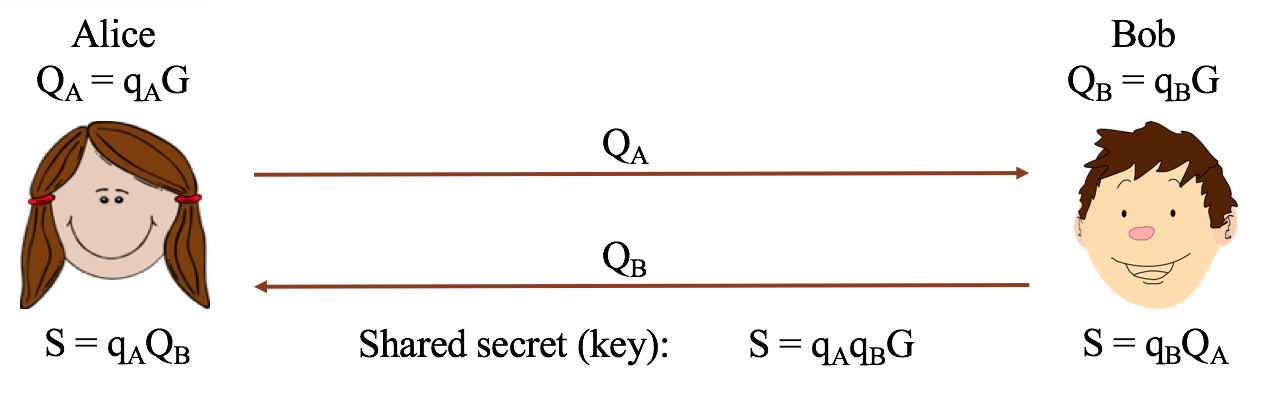
\includegraphics[scale = 0.55]{Images/ECDH.png}
	\captionof{figure}{ECDH key exchange}
	\label{fig:ECDH}
\end{center}
The \textit{setup} phase defines the choice of the elliptic curve domain parameters.\\
The \textit{key deployment} phase requires both parties establishing valid private-public key pairs $(q_A,Q_A)$, $(q_B,Q_B)$ and exchanging their public keys $Q_A$ and $Q_B$ (with further assurance of the public keys being valid ones).\\
The \textit{key agreement} operation defines a way to obtain shared keying data from a shared secret by means of a suitable key derivation function. Observe, however, that the keying data might not directly be used as a key, this just depends on the application.\\ The algorithm below refers to the generation of the shared key by Alice. Bob's algorithm is straightforward and just requires rearrangement of the parameters. We first describe the key derivation function (KDF), taking as inputs an octet\footnote{to keep it simple we can consider an octet being equivalent to a byte.} string $Z$ derived from the field element $z \in \mathbb{F}_n$ outputted by the ECDH primitive\footnote{for more details on the \textit{field-to-octet} conversion, see \cite{Sec}.}, the integers \textit{keydatalen}, \textit{hashlen}, \textit{hashmaxlen} which refer to the length in octets respectively of shared key, hash values and maximum lenght of messages that can be hashed with the given hash function. It outputs a shared key $K$ (octet string) or ``invalid". 
\begin{algorithm}
	\caption{Key Derivation Function}
	\label{alg:KDF}
	\begin{algorithmic}[1]
		\Procedure{kdf}{$Z, \ keydatalen, \ hashlen, \ hashmaxlen $}
		\State assert $|Z| + 4 < hashmaxlen $, ``invalid"
		\State assert $keydatalen < hashmaxlen * (2^{32} -1) $, ``invalid"
		\State $count \gets 1 $  \Comment{4 octet, big-endian string}
		\For {$i\gets 1, \lceil{keydatalen /\ hashlen}\rceil$}
		\State $K_i \gets hash(Z||count)$
		\State $count \gets count + 1$
		\State $i \gets i + 1$
		\EndFor
		\State $K \gets K \verb|>>=| (keydatalen - hashlen)$ \Comment{leftmost keydatalen octects of $K_1||\dots||K_{\lceil{keydatalen /\ hashlen}\rceil}$}
		\State \textbf{return} $K$ 
		\EndProcedure
	\end{algorithmic}
\end{algorithm}\\
Thus, the whole key agreement operation requires deriving a shared field element $z \in \mathbb{F}_n$ by running an instance of the ECDH primitive, converting it to an octet string to give as input to the KDF and consequently deriving a shared key.\\
For what concerns security arguments, it is required the ECDHP (elliptic curve Diffie-Hellman problem) to be hard to solve. It comes out it is closely related to the ECDLP, a third party willing to break it has to solve either $q_A = \log_G{Q_A}$ or $q_B = \log_G{Q_B}$. Consequently, provided a care choice of the parameters during the setup phase, the more powerful algorithms to break it are basically the same presented above for the ECDLP ($\sim O(|\mathbb{G}|^{\frac{1}{2}})$ steps). What that means practically is that with an elliptic curve group order higher than $2^{160}$ (i.e. $160$ bits)\footnote{bearing in mind that, as a rule of thumb, security levels of more than 80 bits are considered satisfactory.} the ECDHP wouldn't be possibly broken.\\ 
Then, another important security assumption relies on the so-called channel authentication for public key exchange, required to prevent \textit{man-in-the-middle} attacks. The latter consist in an adversary eavesdropping over the channel and substituting Alice and Bob's public keys with his own public keys. If the channel is not authenticated\footnote{where authentication means that the recipient has strong reasons to believe that the communication is in place with the ``designated" sender and can be achieved by means of some protocols we do not present here.}, this would prevent Alice and Bob being aware of sharing a secret with the eavesdropper rather than themselves.
\chapter{Confidential transactions}
\label{chpr:CTs}
The aim of this chapter is to present the construction of a \textit{confidential transaction}; in particular, we will see how the cryptographic primitives presented in the previous chapter are deployed (or specialized) and we try to give an overview of benefits and downsides.\\
For this reason we will initially see how a confidential transaction achieves value privacy by encrypting the output amounts through Pedersen commitments and we will describe all of the consequences of homomorphic encryption with an impact on the way confidential transactions are built; then, we will add the range proofs to the scheme, which prevent a malicious transaction's creator to exploit modular arithmetic (and encryption of values) to build invalid transactions in an undetectable way. These proofs are provided in Zero-Knowledge through a particular variant of ring signature. Then, we will enter in the details of the communication between transaction's sender and receiver. Indeed encryption would prevent even the receiver to know the amount associated to each output; thus, some sort of communication is necessary.\\
We conclude the chapter stressing the stunning fact that this whole construction can be obtained without requiring any new cryptographic assumption with respect to the ones already securing Bitcoin; on the other side, we recap its disadvantages.

\section{Transaction amount encryption}
\label{sec::tx_am_encr}
Confidential transactions achieve their goal of obscuring output amounts by replacing output amounts in the clear (Bitcoin-like) with Pedersen commitments to the output amount. This results in substituting the 8-byte integer representing the output amount in a standard Bitcoin transaction with a 33-byte commitment to the amount. Indeed, recalling Definition \ref{Pedersen_commitment}, Pedersen commitments are nothing else than elliptic curve points (the co-domain of the mapping being the elliptic curve group $\mathbb{G}$) which in compressed form can be represented by a 33-byte sequence.\\
On the basis of the previous description of the cryptographic primitive in section \ref{subsec_PC}, this section will be devoted first of all to its transposition in confidential transactions.\\
As an example, we start describing a step-by-step possible strategy to obtain safe encryption of the amounts which culminates in having amounts coded by Pedersen commitments. At each step, we will present pros and cons of the considered solution.\\
Consider a standard transaction with 2 inputs and 2 outputs. The ``balance" of such a transaction in Bitcoin would be represented by the following equation: $v_{i1} + v_{i2} = v_{o1} + v_{o2}$ (where $i$ stands for input, $o$ stands for output). While allowing easy verification that no money has been created out of thin air, such a representation lacks of confidentiality. Next step could be embedding $vH$ in a transaction rather than $v$ only: $v_{i1}H + v_{i2}H = v_{o1}H + v_{o2}H$. Indeed, being $H$ an elliptic curve generator (refer to section \ref{subsec_PC} for details) the equality holds and verification is still easily guaranteed to work. However, this solution suffers from the number of values $v$ being finite and thus from the possibility of an attacker trying to guess the data underlying the commitment. Moreover, observe that knowing $v_iH$ would unmask all of the outputs of value $v_i$ across the blockchain. The final solution to these issues consists in keeping the skeleton of the previous proposal, but blinding the committed value via a random factor, thus effectively coding the amounts through Pedersen commitments: $(r_{i1}G + v_{i1}H) + (r_{i2}G + v_{i2}H) = (r_{o1}G + v_{o1}H) + (r_{o2}G + v_{o2}H)$. In this case the verification of the balance of the equation is guaranteed by the additively homomorphic property stated above, its perfectly hiding nature preserves the confidentiality.\\
The interpretation of the parameters $r$ and $v$ should be now immediate: $r$ represents the secret random \textit{blinding factor}, $v$ represents the committed amount. Thus, in confidential transactions the Pedersen commitment commits to an amount $v$ and requires a random blinding factor $r$ (a private key basically) to obtain the security property of perfect hiding. Each committed amount $v$ and blinding factor $r$ (one per input/output) has to be known only to participants in the transaction; the whole commitment $C$ has to be public instead.

\subsection{NUMS generators construction}
\label{sec::NUMS_gen}
Pedersen commitments are built through nothing-up-my-sleeves (NUMS) generators. On the one hand, generator $G$ has not a clear origin (it is not NUMS in principle); on the other, the Bitcoin protocol specification does not define a second generator associated to the curve.\footnote{The elliptic curve Bitcoin uses is the so called secp256k1, which is a 256-bit elliptic curve over the finite field $\mathbb{F}_p$ and the specification defines the tuple of parameters $T$ = $(p, a, b, G, n, h)$ among which generator $G$, but not generator $H$.}\\
The problem becomes to construct one satisfying Definition \ref{NUMS}. After all, the consequences of having a second generator $H$ not properly built would be catastrophic, because it would make possible to open the commitment to a different value (possibly inflating the currency), tampering with its binding property.\\
For instance, consider the case in which the second generator $H$ is chosen by a malicious designer who knows the (elliptic curve) discrete logarithm with respect to $G$, i.e. he knows $r_H$ such that $H = r_HG$. Thus, $C = rG + vH = rG + vr_HG$. In such a case, it is easy to produce an example in which a commitment to a value $v$ is effectively opened to a different value $v'$. It would be sufficient to make a commitment to a value $v$, $C_v = rG + vH = (r + vr_H)G = ((r - (v'-v)r_H) + v'r_H)G$ and then make the same commitment commit to value $v'$ by publishing $\hat{r} = (r - (v'-v)r_H)$ instead of $r$ as blinding factor. Indeed, $C_{v'} = (\hat{r} + v'r_H)G$ turns out to be a commitment to value $v'$. It is clear instead that he would be unable to use the same trick without knowing $r_H$.\\
The way such a problem could be generically solved\footnote{See for instance \url{https://crypto.stackexchange.com/questions/25581/second-generator-for-secp256k1-curve}.} is by picking $H$ through the hash of an encoding of generator $G$ (of its x-coordinate in particular) and coercing the hash to a curvepoint. Indeed, just hashing the generator could not be sufficient as it couldn't possibly result in obtaining a curve point. In such a case, it suffices to keep on incrementing the obtained hash-value until getting a valid curve point. Confidential transactions exploit this technique. To conclude, it is worth to notice that being the procedure to build the second generator public (and consequently being $H$ hardcoded and available) is not a sufficient condition to deduce the elliptic curve discrete logarithm as at least hashing operations are involved.

\subsection{Explicit fees}
\label{sec::explicit_fees}
Although we need some more steps to figure out completely how a confidential transaction is built, the reader could have possibly already raised an issue with respect to the way fees are managed in such a design.\\
Indeed if one thinks to a standard Bitcoin transaction, fees are what comes out from the difference of amounts associated to transaction inputs and transaction outputs\footnote{Recall that $\sum_i TxO_i + fee = \sum_i TxIn_i$.} and can be easily deduced being the amounts associated to inputs and outputs public.\\
In confidential transactions, the encryption of amounts effectively prevents the same mechanism to work. Not being possible to deduce the fee amount $f$ implicitely, this is explicitely published as a 4-byte plaintext.\\
In turn this has consequences on the commitment scheme. Being fees paid ``unmasked", a Pedersen commitment to fee amount is conceived as $C_f = fH$, rather than $C_f = rG + fH$. Indeed, there's no need to blind anything and it is built with blinding factor $r_f=0$.\\
For what concern transaction propagation, nodes will just check that $\sum_i C_i^{inp} - \sum_i C_i^{out} - fH = 0$ holds, before propagating the transaction further.

\section{Homomorphic encryption features}
\label{Homom_encryption_features}
It turns out that the additively homomorphic property of the Pedersen commitment plays a key role in the design of confidential transactions. In particular it affects the very first issue that one could think of when speaking of confidential transactions, namely how can transaction verification happen. Indeed, as by Proposition \ref{PC_properties}, Pedersen commitment is additively homomorphic in both inputs and it is exactly this property to still allow easy verification of the validity of a confidential transaction\footnote{Despite inputs/outputs amounts not being public.}. What this means is that considering a transaction with 2 inputs and 2 outputs, the following holds: $v_{i1} + v_{i2} - v_{o1} - v_{o2} = 0 \leftrightarrow C_{i1} + C_{i2} - C_{o1} - C_{o2} = 0.$   \\
Then it also affects the way blinding factors are set.

\subsection{Commitment to value 0 \& network verification}
\label{commitment_to_0}
As mentioned, the nodes of the network would verify the validity of a transaction and would eventually propagate it by checking whether the commitments to inputs and outputs sum to 0.\\
On the other hand the additively homomorphic property ensures that having a sum of commitments to a total value of 0 is just the same as having a single commitment to $v=0$ (although such a commitment will never appear). Given that, we anticipate here a result that would be fundamental when we will deal with ring signatures in confidential transactions.\\
A commitment to value $v = 0$ gives the opportunity to create a digital signature with that commitment as though it was a public key (and $v=0$ is special in this sense, you cannot do it with commitment to $v \neq 0$). Indeed, given $C = rG + \cancel{vH}_{v=0} = rG$ you can produce a digital signature with $C$ as verification public key and $r$ as the corresponding private key. Instead, if $v \neq 0$, you would be stuck not knowing the elliptic curve discrete logarithm of $C$ with respect to $G$ because of the addition of $vH$ (i.e. basically because of the NUMS hypothesis on the generator points): $C = rG + vH \rightarrow \underbrace{?}_{unknown} = \log_GC$.\\
At first sight the previous paragraph can be puzzling, but recall that\footnote{As successfully explained in \url{https://bitcoin.stackexchange.com/questions/54042/how-does-a-range-proof-bound-lower-at-0-and-not-1}.} it is only possible to create a digital signature with a point which is a multiple of $G$. By definition, a signature with private key $q$ can be verified with public key $qG$; if $v \neq 0$, it is impossible to find $q$ such that $qG = rG + vH$ as it would require knowing the ratio (i.e. the elliptic curve discrete logarithm) between $G$ and $H$.\\
Eventually, this means that a way a Pedersen commitment can be proven to be a commitment to $v=0$ consists in signing a transaction with the commitment as public key (the message signed is the hash of this commitment public key so as to bind the signature to the commitment), the blinding factor as private key.

\subsection{Blinding factors setting}
\label{sec::blinding_factors_setting}
Being the Pedersen commitment homomorphic in both inputs by Definition \ref{additively_homo_def}, this has a consequence on the way blinding factors are managed: in order for all the commitments in a confidential transaction to sum to 0, not only committed values, but also blinding factors need to sum to 0.\\
Consider as an example the usual transaction with 2 inputs and 2 outputs and let Alice be the sender and Bob the receiver. Suppose moreover that Bob will receive a transaction output only, the other coming back to Alice as change.\\
In such a situation, blinding factors from the inputs are already set as they are associated to commitments to the transaction outputs referenced by the actual transaction inputs. Let's say they are $r_A$, $r_B$. Thus, Alice is left with one degree of freedom in choosing $r_C, r_D$ (the ones associated to the outputs) correctly. For instance she could set $r_C$ as $r_C = r_A + r_B - r_D$ (or she could do the same with $r_D$). Then she will send $r_C$ to Bob\footnote{The safe transfer of blinding factors will require a section on its own.}, which is the blinding factor associated to the commitment to the transaction output he will obtain, but without $r_A, r_B, r_D$ being disclosed.\\
At first sight, such a construction seems to have a security flaw. Indeed, in the example above Alice knows the blinding factor associated to the transaction output sent to the receiver (and in a more general example he would know all of the blinding factors associated to transaction outputs), which would give her the possibility to spend this output. Though observe that here we are just describing the skeleton of a confidential transaction, while not specifying the conditions for spending as they are specific to the different protocols exploiting confidential transactions.\\
In \cite{MW, PoeMW} the issue is addressed by allowing all the commitments to inputs and outputs in a transaction to sum to a non-zero value $kG$, $k$ being the so-called \textit{excess value} (another private key, but chosen by the recipient). This in turn still allows the verification of the validity of the transaction. Indeed, the total amount $v$ of the transaction is still null, which according to section \ref{commitment_to_0} enables to provide a signature with the commitment as public key. Therefore, each Mimblewimble transaction will even include a digital signature provided with the excess blinding factor as private key.\\
On the other hand, this would prevent Alice to be able to spend Bob's output(s).

\section{Zero-Knowledge range proofs}
\label{sec::ZK_range_pr}
The tremendous potential of homomorphic encryption does not come without flaws when applied to Bitcoin. Since the mathematics underlying commitments occurs over a finite field, addition is modular and wraps around: $a + b = c \mod{n} \rightarrow a + b = c + kn$.\\
More precisely, the elliptic curve group $\mathbb{G}$ is cyclic having prime order $n$ (which is a 256-bits prime number) which implies that the outlined scheme based on verifying whether Pedersen commitments to transaction amounts sum to 0 is insecure without additional measures. What can happen is that addition of large values can overflow (indeed a small amount can be in the same equivalent class, modulo the field order, of a very large positive amount) or that negative values can succeed in providing a valid transaction. As a consequence, overflow can basically allow to print an unlimited amount of coins illegally and in such a way that it would be impossible to discover. On the other hand if negative amount were valid, it would be possible to create coins from nothing.\\
As a simple example, yet far from real parameters, overflow can work this way. Consider to have a curve with prime order $n = 13$ and a standard 2 inputs - 2 outputs transaction.
\begin{center}
	\noindent
	\makebox[\textwidth]{
		\begin{tabular}{|c|c|}
			\hline
			Inputs & Outputs \\
			\hline
			$C(1,r_A)$ & $C(8,r_C)$ \\
			\hline
			$C(1,r_B)$ & $C(7,r_D)$ \\
			\hline
		\end{tabular}
	}\captionof{table}{Modular addition: example of wrapping}
	\label{table:wrapping}
\end{center}
In such a situation, matching of input and output commitments yields 0 (1 + 1 - 8 - 7 = -13 $\mod{13}$ = 0), thus the network would validate it. Meanwhile the majority of the coins (13 of 15) has been created illegally.\\
For what concerns the negative-amount-like behaviour, the following could happen:
\begin{center}
	\noindent
	\makebox[\textwidth]{
		\begin{tabular}{|c|c|}
			\hline
			Inputs & Outputs \\
			\hline
			$C(1,r_A)$ & $C(5,r_C)$ \\
			\hline
			$C(1,r_B)$ & $C(-3,r_D)$ \\
			\hline
		\end{tabular}
	}\captionof{table}{Modular addition: negative-amounts}
	\label{table:negative_amounts}
\end{center}
Again, the transaction is still well balanced, there's a creation of coins from nothing and no easy detection (even if $v$ is negative, $vH$ is a usual elliptic curve point).\\
The introduction of Zero-Knowledge range proofs is thus required to prevent wrapping: these configure basically as additional pieces of data which prove each commitment being genuine. In particular, range proofs are a cryptographic tool proving that each committed output is within a certain range ensuring that no overflow is possible and amounts are non-negative (e.g. [$0,2^{32}$) satoshis. Moreover, they are Zero-Knowledge proofs of knowledge and so they prove the committed amount is in range without disclosing neither the amount nor the blinding factor.\\
Two main approaches to range-proof construction are available in literature. This work concentrates on the first solution to the problem, which exploits a particular variant of ring signatures, \textit{Borromean ring signatures} (\cite{Borromean}). In recent times, a new and more efficient solution, \textit{Bulletproofs} (\cite{Bulletproofs}), has come out.

\subsection{Enforce zero-knowledgeness: ring signatures}
\label{example:ZK}
A basic example can motivate the need for providing such a proof in Zero-Knowledge.\\ 
Suppose Alice, the prover, wants to prove to Bob that $C$ is a commitment to the value $v=1$, without telling him the blinding factor $r$, but the value being known.\\
What Bob (the verifier) can do is to compute $C' = C - 1H$\footnote{Recall that $C$ is public and this would just be a point addition operation on the curve.} and ask Alice to provide a signature (with respect to $G$) with public key $C'$. If Alice is able to provide a valid one, then $C$ has to be a commitment to $v=1$. Indeed from section \ref{commitment_to_0}, we know that it is possible to provide a digital signature with the commitment as public key only with commitments to $v=0$. If $C$ is a commitment to $v=1$, then $C'= C - 1H = rG + \cancel{1H} - \cancel{1H} = rG$ (from which $C = rG + 1H$) and Alice knows the blinding factor $r$ to sign with $C'$ as it is the one she has set for the commitment $C$.\\
However, the exposition of the amount would be detrimental to the fulfillment of value privacy, which is the primary purpose of confidential transactions. From here the need to enforce zero-knowledgeness by avoiding giving away the amount. It turns out that this issue can be efficiently approached through ring signatures and next sections will explain how.

\subsection{Role of ring signatures in confidential transactions}
\label{role_ring_sign_in_CT}
In section \ref{ring_signatures} we have described what ring signatures were born for, namely hiding signer's identity in a group of potential signers. However, this is not the only application for which ring signatures can be useful. For instance, in confidential transactions the use of ring signatures is somehow specialized due to their intrinsic nature.\\
Rather than hiding the transaction creator among a group by signing the transaction with a ring signature, in confidential transactions ring signatures will be used to prove that single bits (or digits, depending on the considered encoding) of the encrypted output amount are in a certain range (e.g. \{0,1\}) without giving away the actual number. In particular, the signer will produce a ring of commitments for each digit of the encrypted output amount. In turn, from the number of overall commitments (after the encoding of the encrypted amount is made public) one can deduce the length in digits of the encrypted amount the whole commitment commits to. For instance, considering a binary encoding, it would possible to build a 3-bits amount with 6 Pedersen commitments (2 per bit) and in turn a 3-bits number can be at most in [0,8). Thus if valid it will prove to be a commitment to a value in that range. More technical details will come in next sections.\\
To have an idea of how this can work let us see how the example of section \ref{example:ZK} can be specialized with ring signatures.\\
This time the proof will not give away the amount. In particular, Alice can prove to Bob that $C$ is \textit{either} a commitment to $v=0$ or to $v=1$, thus it is in range $\{0,1\}$.\\
While Alice provides a ring signature over \{$C, C'$\}, Bob can compute again $C' = C - 1H$. If compared with the example in section \ref{example:ZK} where the committed value was known, this time it should be less clear the reason why Bob would compute the same quantity as before. However a single ring with two commitments only should suggest a binary encoding for the committed amount, thus motivating the choice. Then,
\begin{itemize}
    \item if $C$ is a commitment to $v=1$, Alice does not know its discrete logarithm (recall what we have said in section \ref{commitment_to_0}), but $C'$ becomes a commitment to $v=0$ of which she knows the discrete logarithm and makes her able to provide a valid signature over the ring;
    \item on the contrary, if $C$ is a commitment to 0, she knows its discrete logarithm, she doesn’t for $C'$;
    \item if $C$ is a commitment to any other amount, none of them commits to $v=0$, thus preventing Alice to be able to sign.
\end{itemize}
Observe that this can work for any pair of numbers or it can even work to process larger rings.

\subsection{AOS ring signatures}
\label{AOS_ring}
Introduced in \cite{AOS} by Abe, Ohkubo and Suzuki (from which they derive the name), they are a particular variant of ring signatures able to gain consistent reductions in size and verification time with respect to earlier ring signatures schemes. It is worth to notice that when used with discrete-log type keys only (because they allow to use both public keys for integer factoring based schemes and the ones for discrete-log based schemes), they yield much shorter signatures with respect to previous ring signature schemes.\\
The design of the ring is basically the same described in section \ref{ring_signatures}, where a ring of $r$ verification public keys requires knowledge of \textit{one} of the corresponding secret private keys. Moreover, given that all of the verification public keys play the same role in verifying the signature, the specific signing key remains secret.\\ 
They provide ``OR proofs": given a ring with $r$ public keys, the ambiguous signer proves to know \{$q_0$ OR $q_1$ OR $\dots$ OR $q_r$\}.\\
Before entering in the details of the full signature algorithm, it is necessary to describe the way a signer can produce a valid signature in a ring, yet not a ring signature. Let the signer be endowed with his private-public key pair $\{q, Q\}$. This single signature generation involves:
\begin{itemize}
    \item picking up a random nonce $k$ $\rightarrow$ $K = kG$;
    \item given the message $m$ to be signed, computing $hash(K||m)$ $\rightarrow$ $e = hash(K||m)$;
    \item signing as follows: $s = k + eq$;
    \item publishing the signature as $(s,e,m)$.
\end{itemize}
In turn, its verification (given $s, e, m, Q$ as inputs) would imply computing $sG - eQ$. Indeed, $sG - eQ = sG - eqG = (s - eq)G = kG = K$; then with $K$ at disposal the verifier could possibly reconstruct $hash(K||m)$ and verify whether it equals $e$ (given as input). If so, the signature is valid. \\
Thus, it can be noticed that it is nothing else than one of the variants of a Schnorr signature (according to \cite{Schnorr}); the transition to a valid \textit{ring signature} would involve chaining these single signatures together and the way this is done is explained through the full signature algorithm.\\
The complete signature algorithm is the following. Let $m$ be the message to be signed, $i$ be the the index corresponding to the verification public key $Q_i$ in the ring and $i^{*}$ the index corresponding to the unique private key. It outputs the signature $\sigma$ for ($m, Q_i$).
\begin{algorithm}[H]
	\caption{AOS ring signature: signature algorithm}
	\label{alg:AOS_sign}
	\begin{algorithmic}[1]
		\Procedure{AOS-sign}{$m, q_i^{*}, Q_i$: $0 \leq i \leq r-1$}
		\State \textbf{Initialization}:
		\State $k_i^{*}$ $\xleftarrow{\text{\$}} \{1, ..., n - 1\}$
		\State $K_i^{*} \gets k_i^{*}G$
		\State \textbf{Forward sequence}:
		\For {$i \gets i^{*}+1,\dots,r-1,0,\dots,i^{*}$}
		\State $e_i \gets hash(K_{i-1}||m||i)$
		\State $s_i\xleftarrow{\text{\$}} \{1, ..., n - 1\}$
		\State $K_i \gets s_iG - e_iQ_i$
		\EndFor
		\State \textbf{Forming the ring}:
		\State $s_i^{*} \gets k_i^{*} + e_i^{*}q_i^{*}$
		\State \textbf{return} ($e_0, s_0, \dots, s_{r-1}$)$\equalscolon \sigma$
		\EndProcedure
	\end{algorithmic}
\end{algorithm}
\noindent
The key points of the algorithm are the following. At first, all of the $s$-values except for the one which effectively closes the ring are forged.\\
Then, in principle the signature would include the complete set of $e$-values and $s$-values $(e_0, s_0, e_1, s_1, \dots, e_{r-1}, s_{r-1})$. However, as $e$-values can be deterministically retrieved once the first $e$-value and all of the $s$-values are published, it suffices to publish $(e_0, s_0, s_1, \dots, s_{r-1})$, an $(r+1)$-dimensional tuple of 32-bytes numbers. \\ \ \\
Instead, the verification algorithm is the following. It takes as input the message $m$, the whole published signature $\sigma$ and the set of verification public keys $Q_i$, $0 \leq i \leq r-1$. It clearly shows that the signature is valid if the computed $e_0$ coincides with the $e_0$ provided as first entry of the tuple $\sigma$.
\begin{algorithm}[H]
	\caption{AOS ring signature: verification algorithm}
	\label{alg:AOS_verify}
	\begin{algorithmic}[1]
		\Procedure{AOS-verify}{$m, \sigma, Q_i: 0 \leq i \leq r-1$}
		\For {$i \gets 0,\dots,r-1$}
		\State $K_i \gets s_iG - e_iQ_i$
		\State $e_{i+1\%r} \gets hash(K_i||m||i+1)$
		\EndFor
		\If {$e_0 = 0$ or $e_0 \geq n$}
		\State \textbf{return} ``false"
		\EndIf
		\If {$e_0 = \sigma[0]$}
		\State \textbf{return} ``true"
		\EndIf 
		\EndProcedure
	\end{algorithmic}
\end{algorithm}
\noindent
The algorithm shows that the procedure obviously starts at the node for which the $e$-value is known. A valid signature will just ensure that one of the private keys corresponding to the set of public keys $Q_i$ has signed without giving any clue on which effectively did.

\subsection{Borromean ring signatures}
\label{sec::Borromean_r_sig}
Introduced in \cite{Borromean}, Borromean ring signatures are a generalization of the AOS ring signature scheme. They generalize the previous construction as they overcome the simple ``OR proofs" and they can represent proofs of knowledge of more general functions (any monotone boolean function is fine) of the signing keys.\\
While the AOS construction chained signatures together to form a ring, here entire rings of signatures are chained together providing a single and more compact structure of the one that would arise from having $r$ ($r$ being now the number of rings) separate AOS structures. Indeed, the use case of the Borromean ring signatures in confidential transactions is the one in which $r$ separate AOS-like structures and consequently $r$ rings of public keys are needed.\footnote{We will enter in the details later in this section. However, we have already given a hint in section \ref{role_ring_sign_in_CT}: basically a ring per digit of the encrypted output amount is needed.} Though we do not enter now in the details of the benefits of Borromean ring signatures, it is worth to notice that they provide a significant space saving for what concerns signature size.\\
The ambiguous signer can now prove to know one of \{$q_{0,0}$ OR $q_{0,1}$ OR $\dots$\} AND one of \{$q_{1,0}$ OR $q_{1,1}$ OR $\dots$\} AND $\dots$ AND one of \{$q_{{r-1},{0}}$ OR $q_{{r-1},{1}}$ OR $\dots$\}, where the first index represents the ring, the second one represents each public key in the ring (the number of public keys in each ring can in principle differ from ring to ring, but in the described construction it will be the same).\\
Thus, a Borromean ring signature configures as a signature on a message $m$ that can be produced by a signer that knows \textit{all} of the private keys of all the rings of verification public keys (one per ring) or by parties knowing all of them.\\
Moreover, it is the way in which Borromean ring signature is designed to make it achieve its compactness, which in turn affects the signature size (a more compact structure in this case means a structure which requires less public keys for verification). If we represent each ring by means of a graphical structure, we can think of it as a graph with nodes, each referring to a public key and labelled by its $e$-value. The AND/OR gate described above is obtained without requiring multiple graphs, but by means of a graph structure made of $r$ rings, with the optimization of pinning a node (e.g. node 0) as a shared node chaining all the rings. The shared node has an ingoing and an outgoing edge per ring, which should be pretty clear given that it closes all of the rings. Eventually, multiple $s$-values are associated to the shared node and they either require a real private key or force a random $e$-value by picking up a random $s$-value (in analogy with the description provided in section \ref{AOS_ring}).\\
A graphical representation can help in figuring out the overall structure. Figure \ref{fig:Borromean_ringg} considers the example of a structure made of 4 rings all closing in $e_0$. Dashed edges represent those for which $s$-values are connected to known private keys.
\begin{center}
\begin{figure}[H]
\hspace{-1.25cm}
\begin{tikzpicture}[->]%,>=stealth',shorten >=1pt]
  \node[draw, circle] (e0) at (0in, 0in)     {$\textcolor{black!100}{e_0}$};
  \node[draw, circle] (e1) at (1.5in, 1in)   {$\textcolor{black!100}{e_{0,0}}$};
  \node[draw, circle] (e2) at (1.5in, -1in)  {$\textcolor{black!100}{e_{0,1}}$};
  \node[draw, circle] (e3) at (-1.5in, 1in)  {$\textcolor{black!100}{e_{1,0}}$};
  \node[draw, circle] (e4) at (-1.5in, -1in) {$\textcolor{black!100}{e_{1,1}}$};
  \node[draw, circle] (e1_bis) at (2in, 1.5in)     {$\textcolor{black!100}{e_{2,0}}$};
  \node[draw, circle] (e1_ter) at (-2in, 1.5in)     {$\textcolor{black!100}{e_{3,0}}$};
  \node[draw, circle] (e2_bis) at (-2in, -1.5in)     {$\textcolor{black!100}{e_{3,1}}$};
  \node[draw, circle] (e2_ter) at (2in, -1.5in)     {$\textcolor{black!100}{e_{2,1}}$};

  % left circle
  \path
    (e0) edge[bend right] node[left] {\tiny{\textcolor{black!100}{$(s_{1,0}, Q_{1,0})$}}} (e3)
    (e3) edge[bend right, dashed] node[right] {\tiny{\textcolor{black!100}{$(s_{1,1}, Q_{1,1})$}}} (e4)
    (e4) edge[bend right] node[left] {\tiny{\textcolor{black!100}{$(s_{1,2}, Q_{1,2})$}}} (e0)
    (e0) edge[bend right] node[right] {\tiny{\textcolor{black!100}{$(s_{3,0}, Q_{3,0})$}}} (e1_ter)
    (e1_ter) edge[bend right] node[left] {\tiny{\textcolor{black!100}{$(s_{3,1}, Q_{3,1})$}}} (e2_bis)
    (e2_bis) edge[bend right, dashed] node[right] {\tiny{\textcolor{black!100}{$(s_{3,2}, Q_{3,2})$}}} (e0);
  % right circle
  \path
    (e0) edge[bend left] node[right] {\tiny{\textcolor{black!100}{$(s_{0,0}, Q_{0,0})$}}} (e1)
    (e1) edge[bend left, dashed] node[left] {\tiny{\textcolor{black!100}{$(s_{0,1}, Q_{0,1})$}}} (e2)
    (e2) edge[bend left] node[right] {\tiny{\textcolor{black!100}{$(s_{0,2}, Q_{0,2})$}}} (e0)
    (e0) edge[bend left, dashed] node[left] {\tiny{\textcolor{black!100}{$(s_{2,0}, Q_{2,0})$}}} (e1_bis)
    (e1_bis) edge[bend left] node[right] {\tiny{\textcolor{black!100}{$(s_{2,1}, Q_{2,1})$}}} (e2_ter)
    (e2_ter) edge[bend left] node[left] {\tiny{\textcolor{black!100}{$(s_{2,2}, Q_{2,2})$}}} (e0);
\end{tikzpicture}
\captionof{figure}{Graphical structure behind Borromean ring signatures}
\source{adapted from \cite{Borromean}}
\label{fig:Borromean_ringg}
\end{figure}
\end{center}
The complete signature algorithm is the following. Let $Q_{i,j}$, $0 \leq i \leq r-1$, $0 \leq j \leq m_i-1$ be the collection of verification public keys. In particular, $i$ indexes each ring (these are $r$ rings to be chained together), while $j$ indexes each public key ($m_i$ public keys per ring in total). Thus, $Q_{i,j}$ represents the $j^{th}$ public key in the $i^{th}$ ring.\\
Moreover, let $m$ be the message to be signed and $\{q_i\}_{i=0,\dots,r-1}$ be the private key\footnote{There's no need to reference the position in the ring with a second index as there is a known private key per ring only.} corresponding to \{$Q_{i,j_i^{*}}\}_{i=0,\dots,r-1}$, $j_i^{*}$ being the index of the signing key of the $i^{th}$ ring. Thus, $Q_{i,j_i^{*}}$ represents the public key in the $i^{th}$ ring whose corresponding private key is the signing one (i.e. the one that closes the ring).
\begin{algorithm}[H]
	\caption{Borromean ring signature: signature algorithm}
	\label{alg:Borromean_sign}
	\begin{algorithmic}[1]
		\Procedure{Borromean-sign}{$m, q_i: 0 \leq i \leq r-1, Q_{i,j}: 0 \leq i \leq r-1$, $0 \leq j \leq m_i-1$}
		\State $M \gets hash(m||Q_{0,0}||Q_{1,0}||\dots||Q_{r-1,m_{r-1}-1})$
		\For {$i \gets 0,\dots,r-1$}
		\State $k_i$ $\xleftarrow{\text{\$}} \{1, ..., n - 1\}$
		\State $j_i^{*}$ $\xleftarrow{\text{\$}} \{0, ..., m_i - 1\}$
		\State $R_{i,j_i^{*}} \gets k_iG$
		\If {$((j_i^{*}+1)$ \% $m_i )\neq 0$}
		\State $e_{i,j_i^{*}} \gets int(hash(M||R_{i,j_i^{*}}||i||j_i^{*}))$
		\State assert $e_{i,j_i^{*}} \neq 0$ and $e_{i,j_i^{*}} < n$
		\For {$j \gets (j_i^{*}+1)$ \% $m_i,\dots,m_i-1$}
		\State $s_{i,j} \xleftarrow{\text{\$}} \{1, ..., n - 1\}$
		\State $e_{i,j} \gets int(hash(M||R_{i,j}||i||j))$
		\State assert $e_{i,j} \neq 0$ and $e_{i,j} < n$
		\State $R_{i,j} \gets s_{i,j}G - e_{i,j}Q_{i,j}$
		\EndFor
		\EndIf
		\EndFor
		\State $e_0 \gets hash(M||R_{0,m_0-1}||\dots||R_{r-1,m_{r-1}-1})$
		\For {$i \gets 0,\dots,r-1$}
		\State $e_{i,0} \gets int(hash(M||e_0||i||0))$
		\State assert $e_{i,0} \neq 0$ and $e_{i,0} < n$
		\For {$j \gets 1,\dots,j_i^{*}$}
		\State $s_{i,j-1} \xleftarrow{\text{\$}} \{1, ..., n - 1\}$
		\State $e_{i,j} \gets int(hash(M|| s_{i,j-1}G - e_{i,j-1}Q_{i,j-1}||i||j))$
		\State assert $e_{i,j} \neq 0$ and $e_{i,j} < n$
		\EndFor
		\State $s_{i,j_i^{*}} \gets k_i + q_ie_{i,j_i^{*}}$
		\EndFor
		\State \textbf{return} ($e_0, s_{i,j}: 0 \leq i \leq r-1$, $0 \leq j \leq m_i-1$)$\equalscolon \sigma$
		\EndProcedure
	\end{algorithmic}
\end{algorithm}
\noindent
The algorithm produces a valid signature for the whole structure, namely it provides a signature of knowledge of the $r$ private keys \{$q_{i}\}_{i=0,\dots,r-1}$ corresponding to public keys \{$Q_{i,j_i^{*}}\}_{i=0,\dots,r-1}$.\\
For what concerns the computation of the $s$-values and $e$-values and focusing on single rings, it can be noticed that in analogy with the AOS construction each edge $i$ from a node labelled with its $e$-value is characterized by a $s_i$ value which is either random or equal to $s_i = k_i + q_ie_i$ and each node with a single incoming and outcoming edge (all but the shared one) has an associated $e$-value of the type $e_i = hash(m||s_{i-1}G - e_{i-1}Q_{i-1})$.\\
On the other hand, the unique node with multiple ingoing and outgoing edges computes the $e$-value as $e_0 = hash(m||s_{0,m_0-1}G - e_{0,m_0-1}Q_{0,m_0-1}||\dots||s_{{r-1},{m_{r-1}-1}}G - e_{{r-1},{m_{r-1}-1}}Q_{{r-1},{m_{r-1}-1}})$ as it closes $r$ rings.\\
Some other remarks would help in explaining the whole algorithm. First of all, notice the concatenation of both ring number and position in the ring into the computation of $e$-values which guarantees the impossibility of moving rings around without breaking the signature. This of course does not apply to the shared node (node 0) as it is common to all rings.\\
For what concerns the message, it is unique for the whole structure, not ring-specific. This shouldn't be surprising if one recalls that the message to be signed is the hash of the commitment. Thus, being the whole chain of rings to commit to a single commitment, this implies the message being unique\footnote{In the AOS ring signature construction each ring commits to a single commitment, thus the message becomes ring-specific.}.
\\ \ \\
Verification happens according to Algorithm \ref{alg:Borromean_verify}. Indexes obviously run as before and the algorithm takes as inputs the message $m$, the whole signature $\sigma$ and the set of verification public keys $Q_{i,j}$, $0 \leq i \leq r-1$, $0 \leq j \leq m_i-1$.\\
Observe that it is much simpler than the signature algorithm. It avoids the two phases of the signature procedure as it does not depend on which signing keys per ring are known (of course because a verifier does not know them).
Before entering in the details of how Borromean ring signatures are effectively deployed, let us evaluate their benefits in the comparison with the equivalent structure made of AOS ring signatures. Indeed, the construction above should have pointed out that a Borromean ring is structurally equivalent to a number of AOS rings chained in a single shared node. Consider $r$ rings and $N$ verification public keys per ring.
\begin{center}
	\noindent
	\makebox[\textwidth]{
		\begin{tabular}{|c|c|}
			\hline
			& Signature size \\
			\hline
			$r$ AOS ring signatures & $r\cdot N + r$ (32-bytes numbers) \\
			\hline
			Borromean ring signature & $r\cdot N + 1$ (32-bytes numbers) \\
			\hline
			$\Delta$ & $\textbf{r - 1}$ (32-bytes numbers) \\
			\hline
		\end{tabular}
	}\captionof{table}{Borromean ring signature: signature size}
	\label{table:Borr}
\end{center}
The Table \ref{table:Borr} summarizes signature sizes and computes the saving obtained via Borromean ring signatures.
First of all, observe that verifying $r$ AOS ring signatures requires $r\cdot N$ $s$-values ($N$ per ring) and $r$ $e$-values (1 per ring) being published. A Borromean ring signature requires instead a unique $e$-value (the shared one), from which one can easily derive the overall saving. Indeed, it is worth to notice that as the number of rings increases the saving becomes significant. For the small structure in Figure \ref{fig:Borromean_ringg} with 4 rings and 3 verification public keys each we get already a $\sim 20\%$ shorter signature.\\ \ \\
\begin{algorithm}[H]
	\caption{Borromean ring signature: verification algorithm}
	\label{alg:Borromean_verify}
	\begin{algorithmic}[1]
		\Procedure{Borromean-verify}{$m, \sigma, Q_{i,j}: 0 \leq i \leq r-1$, $0 \leq j \leq m_i-1$}
		\State $M \gets hash(m||Q_{0,0}||Q_{1,0}||\dots||Q_{r-1,m_{r-1}-1})$
		\For {$i \gets 0,\dots,r-1$}
		\State $e_{i,0} \gets int(hash(M||e_0||i||0))$
		\If {$e_{i,0} = 0$ or $e_{i,0} \geq n$}
		\State \textbf{return} ``false"
		\EndIf
		\For {$j \gets 0,\dots,m_i-1$}
		\State $R_{i,j+1} \gets s_{i,j}G - e_{i,j}Q_{i,j}$
		\If {$j \neq m_{i}-1$}
		\State $e_{i,j+1} \gets int(hash(M||R_{i,j+1}||i||j+1))$
		\If {$e_{i,j+1} = 0$ or $e_{i,j+1} \geq n$}
		\State \textbf{return} ``false"
		\EndIf
		\EndIf
		\EndFor
		\EndFor
		\State $e_0^{'} \gets hash(M||R_{0,m_0-1}||\dots||R_{r-1,m_{r-1}-1})$
		\State \textbf{return} $e_0^{'} = e_0$
		\EndProcedure
	\end{algorithmic}
\end{algorithm}
\noindent
This section ends with the explanation of how Borromean ring signatures effectively provide Zero-Knowledge range proofs. Their role was previewed in section \ref{role_ring_sign_in_CT}.\\
We have already defined range proofs as additional pieces of data attached to each transaction output proving that the committed output amount lies in a predetermined range of positive values. The first point that needs clarification is the definition of what a proper range would be. This depends on the kind of range proof exploited (in terms of bits of randomness one wants to achieve). For instance, a standard 32-bit range proof limits to a range in between 1 and $2^{32}-1$ satoshis (42.94967295 BTC). However this in principle does not prevent larger outputs to be created, both because any value in between 2 and 64 bits of randomness can be chosen (provided the relative range is made public) and because confidential transactions even support scaling the amount by a power of 10. This latter feature means that provided it is specified that the proof does not deal with satoshi units, but rather with multiples of them, it is possible to process amounts in higher ranges through small proofs.\footnote{As explained in \url{https://bitcoin.stackexchange.com/questions/46865/confusion-of-confidential-transactions}.} For instance referring to the above 32-bit proof, dealing with $10^6$ satoshis as unit, it would be possible to embed all possible amounts ranging in between 0.01 and 42949672.95 BTC. \\
It is also clear that it is even possible to use large ranges for small proofs, but this would make the proof slower to create and verify and it would even imply higher fees.\\
Then it comes the time for the sender to effectively build a range proof per transaction output. As first step, this implies considering the committed output amount (in a given encoding) and ring-signing (with a Borromean-style ring signature) over each digit. The encoding chosen by confidential transactions for the output amount is a base-4 encoding and the reason behind such a choice is that it minimizes the overall number of commitments sent.\\
We start by building the range proof step by step, then we will justify the base-4 representation. For simplicity of notation we consider the 32-bit range proof described above. The procedure is the following:
\begin{itemize}[leftmargin=*]
    \item consider the \textit{output amount} in its \textit{base-4 expansion};\footnote{A 32-bits number can be represented with 16 digits in base-4.}
    \begin{equation*}
        v = v_0\cdot 4^0 + v_1\cdot 4^1 + v_2\cdot 4^2 + \dots + v_{15}\cdot 4^{15}.
    \end{equation*}
    \item \textit{Ring-sign over each digit}, which implies:
    \begin{itemize}
        \item committing through a Pedersen commitment to each digit value, i.e. building $C_i = r_iG + v_i4^iH$, $i=0,\dots,15$, making sure that the sum of commitments is exactly $C$, the commitment to the value associated to the transaction output;
        \item ``arranging" 16 rings of signatures (one per digit) with 4 verification public keys per ring, each committing to one digit value $v_i$ in $0,\dots,3$; 
        \item providing (for each digit) a Borromean ring signature over the ring
        \begin{equation*}
            \{r_iG + v_i4^iH, r_iG + v_i4^iH - 4^iH, r_iG + v_i4^iH - 2\cdot4^iH, r_iG + v_i4^iH - 3\cdot4^iH\}.
        \end{equation*}
        Thus on the one hand each ring proves each digit to commit to a value $v_i\cdot4^i$, $i=0,\dots,3$ (without knowing which one), from which it should be clear that the resulting Borromean ring signature proves the whole commitment to range in $[1, \sum\limits_{i=0}^{15}v_i\cdot4^i]$ satoshi. On the other hand, if $v_i \notin \{0,1,2,3\}$ none of the commitments would be a commitment to $v_i=0$, thus preventing the ring to be signable according to the arguments given in section \ref{commitment_to_0} and to the example presented in section \ref{role_ring_sign_in_CT}.
    \end{itemize}
    \item \textit{Publish} the \textit{range proof} associated to the transaction output.\\
    Notice that according to the outlined scheme, it consists of the set of commitments to each digit value $v_i$ plus the whole Borromean signature:
    \begin{equation*}
        RP_v = (C_0, \dots, C_{15}, \underbrace{e_0, s_{0,0}, \dots, s_{0,3}, \dots, s_{15,0}, \dots, s_{15,3}}_{signature}),
    \end{equation*}
    where as usual the indexes of the $s$-values respectively refer to ring number and position in each ring. 
\end{itemize}
For the sake of clarity we can show a concrete example of the whole procedure.\\
Consider a transaction output of 2,010 BTC (i.e. $201000000_{10}$ satoshi $\leftrightarrow$ $0023332300101000_4$ satoshi).\\
Then, commit to each digit value of the encoded amount through a Pedersen commitment $C_i = r_iG + v_i4^iH$. For instance, considering the third digit from the left (which is a 2), it would mean building the following:
\begin{equation*}
    C_{13} = r_{13}G + 2\cdot4^{13}H = r_{13}G + 134217728H.
\end{equation*}
Then arrange the following set of public keys (for the considered digit):
\begin{align*}
        C_{13,0} &= C_{13} - 0H\\ 
        C_{13,1} &= C_{13} - 1\cdot4^{13}H = C_{13} - 67108864H\\
        C_{13,2} &= C_{13} - 2\cdot4^{13}H = C_{13} - 134217728H\\
        C_{13,3} &= C_{13} - 3\cdot4^{13}H = C_{13} - 201326592H
\end{align*}
Eventually provide a Borromean ring signature over this ring, which in the background means to perform a real signature for $C_{13,2} = r_{13}G$.\\
For what concerns the range proof size, consisting of the shared $e$-value, 4 $s$-values per ring and a commitment per ring it is about 2.6 KB per transaction output. Given these premises, it can also be proven that the base-4 representation minimizes the total size of the range proof.\\
Indeed, given that $y$ is the number of bits-per-digit in each encoding\footnote{Base 2 $\leftrightarrow$ 1 bit per digit; base 4 $\leftrightarrow$ 2 bits per digit; base 8 $\leftrightarrow$ 3 bits per digit etc.} and given that we are considering 32-bit range proofs, it can be proven that the total number of commitments plus $s$-values (the $e$-value is unique independently of the encoding) is given by $N(y) = \frac{32}{y}\cdot(1+2^y)$.
\begin{center}
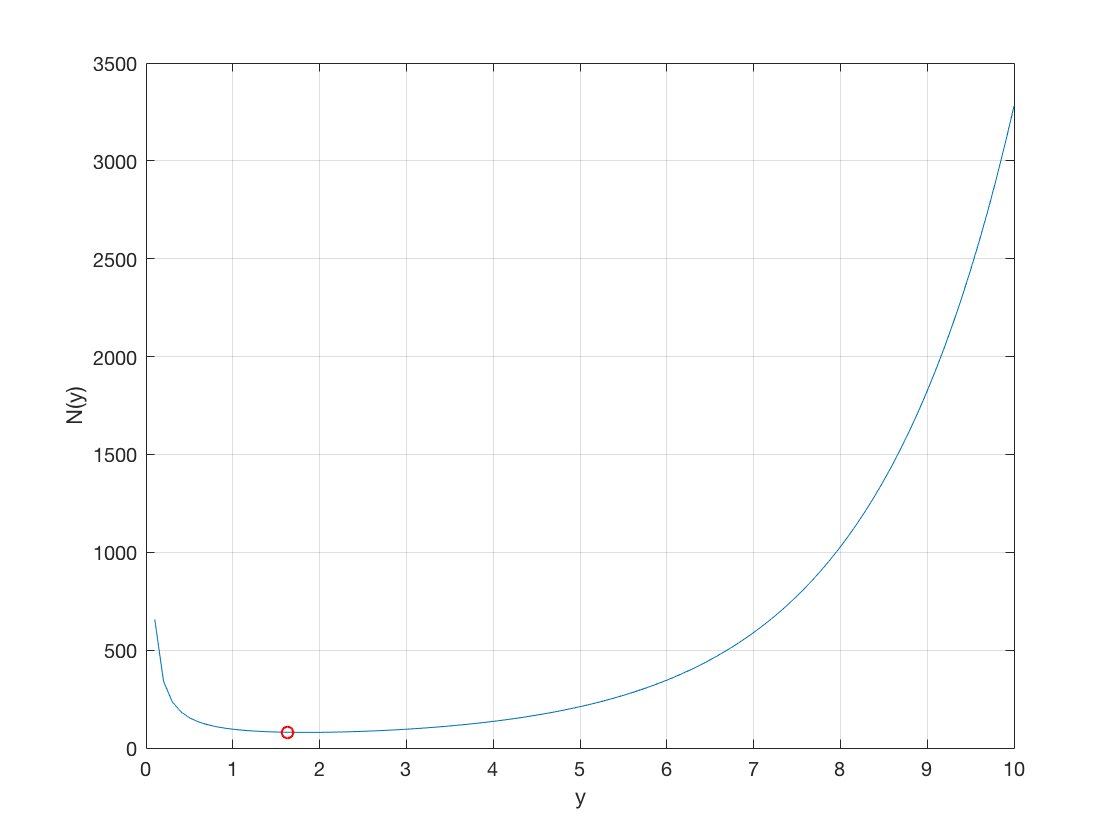
\includegraphics[scale = 0.25]{Images/N_y.png}%
\captionof{figure}{Total number of commitments plus s-values}
\label{fig:N_y}
\end{center}
As Figure \ref{fig:N_y} shows, $N(y)$ takes its minimum around $y=2$, meaning that the minimization occurs when considering the base-4 encoding.

\section{Sender/receiver communication}
\label{sender_recv_comm}
What is left out are the details about the communication between sender and receiver for what concerns setting of the blinding factors and transmission of the committed amounts. Indeed, from the point of view of the network range proofs represent proofs that output amounts are valid, but amounts (together with blinding factors) stay secret as they are blinded by Pedersen commitments. However, both amounts and blinding factors need to be known by participants in the transaction. This opens the issue of their safe transfer from sender to receiver.\\
It turns out that confidential transactions succeed in providing a space-saving solution to embed these secret data in the transaction without adding more data rather than commitments and range proofs. Indeed, \textit{amounts} are embedded in range proofs without taking up more space; \textit{blinding factors} can be retrieved by sender and receiver only as part of a deterministic generation process which enables the transfer to happen non-interactively.\\
In addition to this, it is even possible to transfer arbitrary user-selected data without further overload.\\
Thus, we will see how the ECDH primitive presented in section \ref{ECDH} is exploited to serve the purpose this section is all about. First of all we recall that an instance of ECDH is needed to define a shared key between sender and receiver.\\
A peculiarity of confidential transactions is that each address contains a \textit{scanning public key} for ECDH purpose only. More precisely, the sender ECDH public key is published as part of the output (it coincides with $Q_A$ in the scheme of section \ref{ECDH}), while each confidential transaction address contains the ECDH public key of the receiver ($Q_B$ in section \ref{ECDH}). Eventually $q_A$ and $q_B$ play the role of ECDH ephemeral private keys (respectively associated to the sender scanning key and the receiver one). Given this, it is clear that both sender and receiver can compute the same secret key as it was described in section \ref{ECDH}.\\ 
The shared key is then used by both sender and receiver to seed a RFC6979 \cite{rfc6979} pseudo-random number generator (prng) to deduce the same blinding factors and random $s$-values which enter in the Borromean ring signature algorithms. Indeed without entering in the details of the RFC6979 standard, this is used to deterministically and safely generate the nonce $k$ to be used in ECDSA signatures and outside ECDSA can basically work as a cryptographically secure pseudo-random number generator taking as input a seed. Moreover, various rounds of RFC6979 can be run in sequence, each time using the previous output as seed.\\
Making this process deterministic, provides some sort of advantages. Among these there is certainly the possibility to distinguish where randomness resides and exploit the feature accordingly. For the \textit{sender}, this configures in the possibility to send the committed transaction output amount (and possibly other kinds of arbitrary selected data) over predetermined and forged signature values (we will describe how in a while); for the \textit{receiver}, this means to possibly ``rewind" the proof and in turn generate the same blinding factors of the sender, read the transaction output amount and extract further messages the sender could have sent.\\
We will enter now in all of these details.
\begin{itemize}[leftmargin=*]
\item \underline{Setting and transmission of the blinding factors}:\\
the 32-bit range proof of the previous section includes a commitment per digit of the committed output amount, the blinding factors of which should be known by the receiver (their sum being nothing else than the blinding factor of the commitment to the output amount). Indeed, 16 blinding factors (one per ring) should be shared by sender and receiver.\\ 
At this extent the 32-byte shared key derived from the ECDH instance is used as first seed to a RFC6979 prng, each successive output is used as next seed to deduce all of the blinding factors $r_0, r_1, \dots, r_{15}$ (though $r_{15}$ is obtained by difference so as to to match the sum of the blinding factors from inputs).
\item \underline{Generation of forged signatures and nonces}:\\
as we have described, in the Borromean ring signature algorithm a single $s$-value per ring is obtained from a known private key, all the others are forged, but indistinguishable from random. In the example of the 32-bits range proof discussed in the previous section, this means that $\frac{3}{4}$ of the $s$-values are forged and again a RFC6979 prng is used to generate them in such a way that the receiver would be able to easily retrieve all of them by seeding the prng with the same seed the sender has used. \\
For what concerns nonces $k$, one per ring is required to be picked uniformly at random. Observe that $k_i$, $i = 0, \dots, r-1$ enters in the computation of the real $s$-value only, meaning that even for the remaining $\frac{1}{4}$ of the $s$-values generation of random values is needed (and the same solution is adopted).
\item \underline{Transmission of committed amount}:\\
the transaction output amount is embedded in the already provided construction in such a way that it is easily available to the receiver and does not occupy more space.\\
Given that the published range proof has to be indistinguishable from random for anybody but the participants in the transaction, after locating where randomness resides ($s$-values that can be retrieved via RFC6979 procedure are the forged ones) the idea is to replace this randomness in the range proof with an encrypted message that the receiver only can decode.\\
In particular, the amount is embedded into one of the forged signatures (usually the last one, unless it is the real one) by XORing\footnote{The XOR is the \textit{bitwise addition} without carry. Among its properties: 
\begin{itemize}
    \item A $\oplus$ 0 = A;
    \item A $\oplus$ A = 0;
    \item (A $\oplus$ B) $\oplus$ C = A $\oplus$ (B $\oplus$ C);
    \item (B $\oplus$ A) $\oplus$ A = B $\oplus$ 0 = B.
\end{itemize}} it with the forged $s$-value for that signature. Indeed, the XOR does not affect the pseudo-randomness of the original $s$-value. Moreover, it could be useful to stress once more the fact that only forged signatures are tampered with in this way; the real $s$-value is necessary to close the ring and validate the signature, so it mustn't be manipulated.\\
Referring to forged signatures only (and consequently forged $s$-values only), let $s_{common}$ be the $s$-value deterministically generated via the RFC6979 procedure and $s_{published}$ be the $s$-value actually published by the sender in the range proof. What this means is that $s_{published}$ is given by
\begin{equation*}
    s_{published} = s_{common} \oplus amount,
\end{equation*}
and implies that: 
\begin{equation*}
    s_{common} \oplus s_{published} = s_{common} \oplus s_{common} \oplus amount = amount.
\end{equation*}
Thus, the receiver by looking at the last $s$-value (unless it is the case that the last $s$-value is not forged) and computing $s_{common} \oplus s_{published}$ sees the amount if the last signature has been tampered with it, 0 if not.
\item \underline{Transmission of other user-defined data}:\\
the amount takes 32 bytes only, all the rest less the space corresponding to real $s$-values (which is however almost 80\% of the size of the range proof) can be exploited in a similar way for the transmission of arbitrary data. These data rather than the amount would be XORed in with the pseudo-random $s$-values. \\
Thus, at least one (if no arbitrary data is sent) of the forged $s$-values published as part of the range proof is the result of a XORing.
\item \underline{Proof's ``rewind" by the receiver}:\\
given the shared key, the receiver can run the same RFC6979 procedure of the sender and in turn deduce same blinding factors and $s$-values. In turn he can perform the XOR operation as it was described before.
\end{itemize}

\section{Benefits and downsides}
\label{sec::final_sec}
Confidential transactions can be possibly constructed without adding any additional cryptographic assumptions with respect to the ones underlying the main protocol: this means that they just require the hardness of the ECDLP. This is quite relevant as it is not that common to add privacy features without relying on harder assumptions.\\
However, what effectively makes confidential transactions (at least in the form presented in this work) not ready yet for integration in the main protocol is the excessive overload on transaction size. The presented solution (which builds range proofs through Borromean ring signatures) requires a proof which is about 2.6 KB per transaction output (with 32 bits of precision), which means a total size of about 5.4 KB (5 KB of which deriving from the range proof) for a typical transaction with two outputs (the transaction size even grows linearly with the number of outputs); too much with respect to a standard Bitcoin transaction.
\\ \ \\
Moreover, confidential transactions are actually implemented in the Elements sidechain.\footnote{See \url{https://github.com/ElementsProject/elements}.} De facto they introduce a different transaction format with respect to the one presented in Chapter \ref{chpr:tx}. Each output includes Pedersen commitment to the output amount, associated range proof, ECDH public key of the sender and locking script. Despite not having presented the details, in section \ref{sender_recv_comm} it was mentioned that they even introduce a new type of address (longer than a standard one) called \textit{confidential transaction address} which includes the ECDH public key of the receiver. The locking script includes the confidential transaction address. \\
A very powerful comprehensive schema can be seen in Figure \ref{fig:ct_schema} and is taken from \cite{GibsonCT}. It represents a confidential transaction with two inputs and two outputs.
\begin{center}
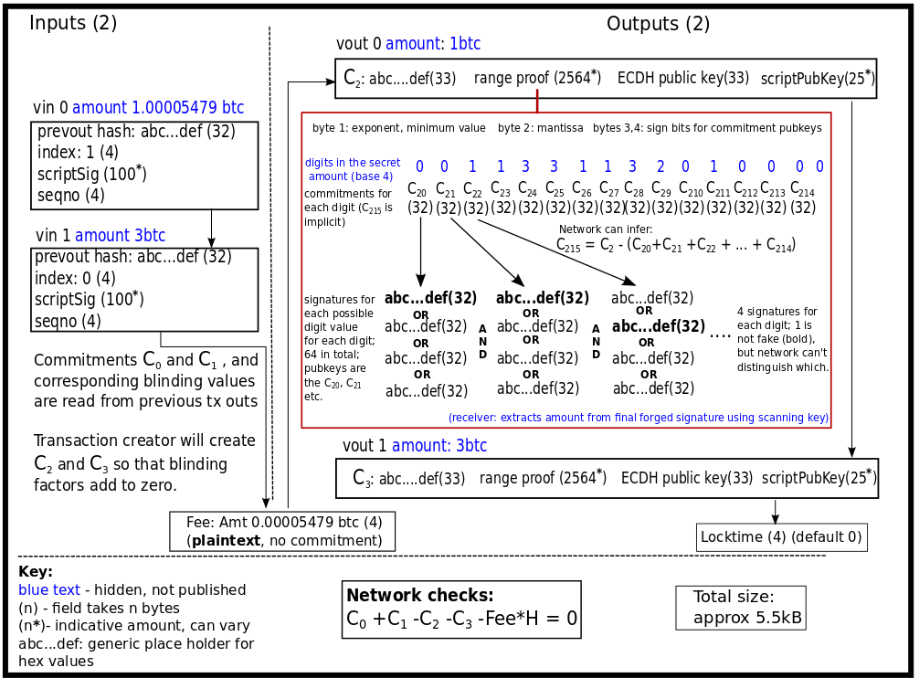
\includegraphics[scale = 0.7]{Images/CT_schema.png}%
\captionof{figure}{Confidential transaction format}
\source{\cite{GibsonCT}}
\label{fig:ct_schema}
\end{center}
%\chapter{Conclusions}
\label{chpr:conclusions}
This thesis has tried to motivate the importance for Bitcoin to adopt technologies enhancing privacy in the incoming years. This would not merely improve the privacy of people transacting (which is indeed fundamental), but even strengthen its ability to serve as money. Indeed, though it cannot be recognized as a good unit of account, Bitcoin is a good store of value (it is durable, it can be reliably saved, stored with low costs and easily retrieved) and an excellent medium of exchange (it is easily portable, divisible, swappable, resistant to counterfeiting). Its greatest lack is that it is not that fungible and it is the case that fungibility is strictly linked to privacy.\\
At the same time, this work should have outlined the reasons why no privacy-based solutions have been soft-forked yet in Bitcoin at the time of writing; this is not certainly for a lack of proposals, quite the opposite. Developers have worked in this direction since long time, but cryptographic, privacy-based solutions are costly and require commitments, thus opening other issues.\\
Moreover, through confidential transactions \cite{Max15} we have explored some nice features of homomorphic encryption applied to commitment schemes, the interesting field of Zero-Knowledge proofs, a fancy variant of digital signature scheme and a clever solution for the communication of transaction amount, blinding factors and other user-selected metadata between participants in the transaction.\\
Confidential transactions basically hides each output amount through a Pedersen commitment to the amount and add a range proof ensuring that the amount does not overflow. The solution we have described builds each range proof through a Borromean ring signature. Among the strengths of confidential transactions, the fact that these can be possibly constructed without new cryptographic assumptions with respect to the main protocol, but relying on the hardness of the ECDLP (differently from some alternative schemes like Zcash's ones) and the substantial savings in terms of size and verification time with respect to previous solutions (which have made them sources of inspiration for privacy-based alt-coins like Monero, that has effectively implemented confidential transactions through ring signatures, RingCT \cite{RingCTMonero}). On the other hand, the solution suffers from the size of the range proof attached to each transaction output (and thus of the entire transaction) being too large.\\
These weaknesses have prevented confidential transactions to be soft-forked in Bitcoin up to now.\\
More recently, however, a new and more efficient solution to range proof construction \cite{Bulletproofs} has been proposed. Its name is Bulletproofs and it is likely worth studying: it could be the solution being effectively soft-forked in the future (it even naturally marries some older proposals) and effectively bringing consistent privacy in the protocol. Indeed, Bulletproofs is still well-suited for constructing efficient range proofs on committed value, but it also adds various optimizations.\\
At first, it provides aggregation of range proofs: it would be possible to prove that $m$ commitments lie in a given range by just providing additional O($\log m$) group elements with respect to a single proof, making it growing logarithmically with the number of transaction outputs. This would be already useful for confidential transactions by themselves as standard Bitcoin transactions have generally at least two outputs and it would even make it efficiently combine with Coinjoin \cite{Max13}. Additionally it could simultaneously double the range proof precision at marginal additional cost.\\
Then, it would allow batched verification of multiple Bulletproofs.\\ All of these enhancements with a total transaction size not so bigger than a standard transaction according to \cite{Bulletproofs,CT_eff}.\\
Moreover, confidential transactions are even beneficial for a newborn and promising cryptosystem called Mimblewimble \cite{MW, PoeMW}. Mimblewimble is still a transaction output based system (thus a Bitcoin-like blockchain system) which however implements confidential transactions from the beginning. At the time of writing it is already being built through Bulletproofs, thus inheriting its benefits. Moreover, Mimblewimble removes the need for the unlocking script because it allows to prove a transaction to commit to a Pedersen commitment to 0 just signing the transaction through the difference of the commitments to outputs and inputs. Other than this, it can benefit from transaction aggregation and enables the construction of a simplified blockchain where spent transactions can be pruned, thus improving scalability.



%----------------------------------------------------------------------------------------
%	THESIS CONTENT - APPENDICES
%----------------------------------------------------------------------------------------

\appendix
\chapter{Abstract algebra fundamentals}
\label{app:A}
This appendix is aimed at providing some fundamental notions of  algebra of sets and number theory at the basis of the considered public-key cryptosystem. Definitions are mainly taken from \cite{UnderstandingCrypto} and adapted when needed.
\section{Groups}
We start from the definition of a \textit{group}.
\begin{mydef} A group is a set of elements $\mathbb{G}$ together with an operation $\circ$ which combines two elements of $\mathbb{G}$. A group  satisfies the following properties:
	\begin{itemize}
		\item The group operation $\circ$ is closed: $\forall a, b \in \mathbb{G} \rightarrow a \circ b \in \mathbb{G}$.
		\item The group operation $\circ$ is associative: $\forall a, b, c \in \mathbb{G}  \rightarrow (a \circ b) \circ c = a \circ (b \circ c)$.
		\item Identity: $\exists e \in \mathbb{G} \ | \ \forall a \in \mathbb{G}, \ e \circ a = a \circ e = a$.
		\item Invertibility: $\forall a \in \mathbb{G}, \ \exists b \in \mathbb{G} \ | \ a \circ b = b \circ a = e$. This element is called inverse of a and it is commonly denoted either as $a^{-1}$ or $-a$, depending on the notation (multiplicative or additive).
		\item A group $\mathbb{G}$ is abelian (or commutative) if, furthermore, $\forall a, b \in \mathbb{G} \rightarrow a \circ b = b \circ a$.
	\end{itemize}
\end{mydef}
\label{defA1}
\noindent
Depending on whether we consider additive or multiplicative notation, the operation $\circ$ stands respectively for addition or multiplication.
\begin{myrem} The group operation $\circ$ is called group law of $\mathbb{G}$.
\end{myrem}
\begin{myrem} The number of elements in a group $\mathbb{G}$ is called group order (or cardinality). We denote it by $|\mathbb{G}|$.
\end{myrem}
\begin{myexample}
$(\mathbb{Z},+)$ is a group. Particularly, it forms an abelian group where $e = 0$ is the identity element, $b = -a$ is the inverse of an element $a \in \mathbb{Z}$.
\end{myexample}
\begin{myexample}
$(\mathbb{Z} \backslash \{0\},\cdot)$ is \textbf{not} a group. Particularly, $\nexists b = a^{-1}$ for an element $a \in \mathbb{Z}$ with the exception of the elements -1 and 1.
\end{myexample}
\begin{myexample}
$(\mathbb{Z}_m,+)$, where $\mathbb{Z}_m$ = $\{0,1,\dots,m-1\}$ and the operation is the addition modulo m, form a group (of order $m$) with the identity element $e = 0$. Every element $a$ has an inverse $b=-a$ such that $a + (-a) = 0$ mod m.
\end{myexample}
\begin{myrem}
This last example points out a straightforward, yet important, fact. By definition, the inverse must belong to the group $\rightarrow$ $b=m-a$ is the inverse of any group element $a$.
\end{myrem}
\begin{myrem}
Observe that $(\mathbb{Z}_m,\cdot)$ is \textbf{not} a group. Most elements $a$ do not have an inverse such that $aa^{-1} = 1$ mod m.
\end{myrem}
\noindent
Actually, in cryptography it turns out that the groups playing a significant role are those with a finite number of elements. We briefly focus now on one of them, $(\mathbb{Z}_m^{*},\cdot)$, the multiplicative group of $\mathbb{Z}_m$.\\
Let's start with some definitions.
\begin{mydef}
    Given $x,y \in \mathbb{Z}$, $gcd(x,y)$ is the greatest common divisor of $x,y$.
\end{mydef}
\label{defA2}
\begin{myrem}
    If $gcd(x,y)=1$, we say that $x,y$ are relatively prime.
\end{myrem}
\begin{mylemma}
    $\forall x,y \in \mathbb{Z}$, $\exists a,b \in \mathbb{Z}$ s.t. $ax+by=gcd(x,y)$. a,b, can be efficiently found through the extended Euclidean algorithm (see \cite{UnderstandingCrypto} for details).
\end{mylemma}
\noindent
Given the definition of inverse element of a group seen above, we introduce the following:
\begin{mylemma}
    $x$ in $(\mathbb{Z}_m,\cdot)$ has an inverse $\longleftrightarrow$ $gcd(x,m)=1$. 
\end{mylemma}
\begin{proof} ($\longrightarrow$) Suppose by contradiction that $gcd(x,m)>1$. Then, $\forall a: gcd(ax,m)>1$ $\rightarrow$ $ax \neq 1$ in $\mathbb{Z}_m$, which (according to \ref{defA1}) contradicts the hypothesis.\\
($\longleftarrow$) $\exists a,b$: $ax + \cancel{bm} = 1$ ($bm = 0$ mod $m$, thus $bm=0$ in $\mathbb{Z}_m$) $\rightarrow$ $ax=1$ in $\mathbb{Z}_m$ $\rightarrow$ $x$ is invertible in $\mathbb{Z}_m$, the inverse being $x^{-1}=a$.
\end{proof}
\begin{myprop}
    $(\mathbb{Z}_m^{*},\cdot)$ = $\{x \in \mathbb{Z}_m: gcd(x,m)=1\}$ forms an abelian group. The identity element is $e=1$.
\end{myprop}
\begin{proof}
    The proof is straightforward and comes from the verification of the group properties described above.
\end{proof}
\begin{myrem}
    In particular, if $m$ is prime, then $\mathbb{Z}_m^{*}$ = $\mathbb{Z}_m \backslash \{0\}$.
\end{myrem}
\subsection{Cyclic groups}
Next step before coming to field structures is to introduce the notion of \textit{cyclic group}, necessary in turn to introduce the Generalized Discrete Logarithm Problem, which is at the basis of ECC.\\
Let's first start with some preliminary definitions.
\begin{mydef}
    A group $(\mathbb{G},\circ)$ is finite if it has a finite number of elements. 
\end{mydef}
\begin{mydef}
    The order $ord(x)$ of an element $x$ of a group $(\mathbb{G},\circ)$ is the smallest positive integer $k$ such that $x^k=1$, $e=1$ being the identity element of $\mathbb{G}$.
\end{mydef}
\begin{myexample}
    In $(\mathbb{Z}_7^{*},\cdot)$, $ord(x=2)=3$. Indeed $2^1$ = $2$ mod $7$, $2^2$ = $4$ mod $7$, $2^3$ = $1$ mod $7$.\\
    It is even interesting to see that by keeping on computing powers of $x=2$, those will keep on running through the above sequence. Indeed, $2^4$ = $2$ mod $7$, $2^5$ = $4$ mod $7$, $2^6$ = $1$ mod $7$.
\end{myexample}
\noindent
Based on this, 
\begin{mydef}
    A group $(\mathbb{G},\circ)$ which contains an element $x$ with maximum order $ord(x)$ = $|\mathbb{G}|$ is said to be cyclic. Elements with maximum order are called generators and are denoted by $g$.
\end{mydef}
\begin{myrem}
\label{generator_spanning}
    The reason for which $g$ is called generator is that it generates (or spans) the entire group (all the group elements can be recovered by raising $g$ to the powers $1,\dots,|\mathbb{G}|$). In the previous example, $g=3$ is a generator.
\end{myrem}
\begin{myrem}
    It is also clear that not every element is a generator of the cyclic group ($x=2$ being an example).
\end{myrem}
\noindent
Then we introduce three more theorems defining fundamental properties of cyclic groups. The first one is the following, by Euler.
\begin{mytheorem}
    For every prime $p$, $(\mathbb{Z}_p^{*},\cdot)$ is an abelian finite cyclic group.
\end{mytheorem}
\begin{mytheorem}
\label{thm::order_divides_cardinality}
    Let $\mathbb{G}$ be a finite cyclic group. Then $\forall x \in \mathbb{G}$, $ord(x)$ divides $|\mathbb{G}|$.
\end{mytheorem}
\noindent
Consequently, in a cyclic group there exist only element orders dividing exactly the cardinality of the group. 
\begin{myrem}
    In the already analyzed $(\mathbb{Z}_7^{*},\cdot)$, the only possible element orders are $ord(x)=1,2,3$ being $|\mathbb{G}| = 6$.
\end{myrem}
\begin{mytheorem}
\label{thm::prime_order_all_gen}
    Let $\mathbb{G}$ be a finite cyclic group. Then, if $|\mathbb{G}|$ is prime, all elements $x \neq 1 \in \mathbb{G}$ are generators.
\end{mytheorem}
\begin{proof}
    By \ref{thm::order_divides_cardinality}, being the group cardinality a prime, the only possible element orders are $ord(x)=1$ or $ord(x)=|\mathbb{G}|$. As $ord(x)=1$ $\longleftrightarrow$ $x=1$, then any $x=g \neq 1 \in \mathbb{G}$ is a generator.
\end{proof}
\noindent
The last needed definition concerning group is the one of \textit{subgroups}, basically non-empty subsets $\mathbb{H}$ of a (cyclic) group $\mathbb{G}$ being themselves groups.
\begin{mytheorem}
    Let $(\mathbb{G},\circ)$ be a cyclic group. Then every element $x \in \mathbb{G}$ with $ord(x)=s$ is the generator of a cyclic subgroup with $s$ elements.
\end{mytheorem}
\section{Fields}
We can eventually introduce the definition of \textit{field}.
\begin{mydef}
    A field $K\neq0$ is a set of elements with the following properties:
    \begin{itemize}
        \item $(K,+)$ is an abelian (additive) group, with identity element $e=0$.
        \item $(K\backslash\{0\},\cdot)$ is an abelian (multiplicative) group, with identity element $e=1$.
        \item The distributivity law holds, i.e., $\forall$ $a,b,c \in K$: $a \cdot (b+c)$ = $(a\cdot b) + (a\cdot c)$.
    \end{itemize}
\end{mydef}
\begin{myexample}
    The set $(\mathbb{R},+,\cdot)$ of real numbers is a field with identity element $e=0$ for the additive group and identity element $e=1$ for the multiplicative group. $\forall a$ $\exists b = -a$ additive inverse, $\forall a\neq 0$ $\exists b =\frac{1}{a}$ multiplicative inverse.
\end{myexample}
\begin{myexample}
\label{prime_finite_field}
    For every prime $p$, the set $(\mathbb{Z}_p,+,\cdot)$ is a field.
\end{myexample}
\begin{myrem}
    \ref{prime_finite_field} shouldn't be much of a surprise, given the premises. Indeed, we have already seen $(\mathbb{Z}_p,+)$ is an additive group; $(\mathbb{Z}_p\backslash\{0\},\cdot)$ in principle ($p$ generic) wouldn't be a multiplicative group, but $p$ prime implies $(\mathbb{Z}_p\backslash\{0\},\cdot)$ $\equiv$ $(\mathbb{Z}_p^{*},\cdot)$, which we have already seen being a multiplicative group.
\end{myrem}
\begin{myrem}
    \ref{prime_finite_field} is also the most common representative of prime finite field, which cryptography is most concerned on.
\end{myrem}
\subsection{Finite fields}
\begin{mydef}
    A finite field is a field with a finite number of elements (also called Galois field).
\end{mydef}
\begin{mytheorem}
    A finite field of order $q$, denoted as $\mathbb{F}_q$, only exists if $q = p^k$, $p$ prime number, $k$ positive integer.
\end{mytheorem}
\noindent
In particular, prime finite fields (\ref{prime_finite_field} being the most representative example) takes a fundamental role in dealing with the DLP, argument of the next section.
\section{Discrete Logarithm Problem}
\label{DLP}
We conclude the appendix with the Discrete Logarithm Problem, in its various formulations.\\
Consider the prime finite field $\mathbb{F}_p$ = $(\mathbb{Z}_p,+,\cdot)$, $p$ prime.\\
It turns out that the DLP can be directly explained through cyclic groups (from which our previous concern in their description). We present it in its multiplicative form (thus DLP over $(\mathbb{Z}_p^{*},\cdot)$), the additive one being simple to recover from.
\begin{mydef}
    Given the finite cyclic group $(\mathbb{Z}_p^{*},\cdot)$, a generator $g \in \mathbb{Z}_p^{*}$ and another element $y \in \mathbb{Z}_p^{*}$, the DLP is the problem of determining the integer $1 \leq k \leq p-1$ such that $g^k = y \mod{p}$. 
\end{mydef}
\begin{myrem}
    Being $g$ a generator of a finite cyclic group and $y$ another group element, $k$ must necessarily exist due to \ref{generator_spanning}.
\end{myrem}
\begin{myrem}
    $k = \log_g{y} \mod{p}$, from which its name.
\end{myrem}
\begin{myrem}
    The obvious transposition to additive groups: determining $k$ such that $kg=y$.
\end{myrem}
\noindent
Here it comes, instead, the reason of the introduction of subgroups.
\begin{myrem}
    It is often desirable to have the DLP in groups where $|\mathbb{G}|$ is prime to prevent the so called Pohlig-Hellman attack\footnote{For security consideration we refer to \cite{UnderstandingCrypto}; the only thing we point out is that the cited one is not the only possible attack (\textit{brute-force search}, \textit{Baby-step giant-step}, \textit{Pollard $\rho$ method} being other possibilities) and that the best known algorithm runs in time $O(|\mathbb{G}|^{\frac{1}{2}})$.}; being $|\mathbb{Z}_p^{*}|=p-1$ (not prime), subgroups of  $\mathbb{Z}_p^{*}$ with $|\cdot|=n$, $n < p$, $n$ prime are usually exploited.
\end{myrem}
\subsection{Generalized Discrete Logarithm Problem}
It is possible to generalize and present the DLP over an arbitrary cyclic group, which is at the basis of ECC.
\begin{mydef}
    Given a finite cyclic group $(\mathbb{G},\circ)$ such that $|\mathbb{G}| = n$, a generator $g \in \mathbb{G}$ and $y \in \mathbb{G}$, the GDLP is the problem of determining the integer $k$, $1 \leq k \leq n$ such that $y = \underbrace{g \circ g \circ \dots \circ g}_{k \quad times}$ = $g^k$.
\end{mydef}
\begin{myrem}
    The same considerations presented before hold here.
\end{myrem}


\backmatter
%----------------------------------------------------------------------------------------
%	BIBLIOGRAPHY
%----------------------------------------------------------------------------------------

\backmatter
\nocite{*}
\bibliographystyle{acm}
\bibliography{Bibliography/biblio}



\end{document}  